\documentclass{article}

\usepackage{fullpage}
\usepackage{parskip}
\usepackage{setspace}
\usepackage{mathtools}
\usepackage{tikz}
\usetikzlibrary{arrows}
\usetikzlibrary{decorations.markings}
\usetikzlibrary{calc}
\usepackage{standalone}
\usepackage{float}
\usepackage{caption}
\usepackage{subcaption}
\usepackage{amsmath}
\usepackage{amsfonts}
\usepackage{amsthm}
\usepackage[ruled]{algorithm2e}
\usepackage{adjustbox}
\usepackage{enumerate}
\usepackage[nocompress]{cite}
\usepackage{hyperref}

\newtheorem{definition}{Definition}
\newtheorem{theorem}{Theorem}
\newtheorem{proposition}{Proposition}
\newtheorem{lemma}{Lemma}
\newtheorem{remark}{Remark}

\title{On Deadlocking in Queueing Networks}
\author{Geraint Ian Palmer}
\date{}


\begin{document}
\onehalfspacing

\maketitle

This report will define and discuss the properties and detection of deadlock in queueing networks.
Throughout the section, when discussing queueing networks, it is assumed that
the queueing network is open and connected.
Open queueing networks are those networks that have at least one node to which customers arrive from the exterior, and least one node from which customers leave to the exterior.

\section{Introduction}

A simple representation of deadlock in the context of road traffic is shown in Figure~\ref{fig:gridlock}.
Here deadlock, or gridlock, is caused by the mutual blocking of vehicles.
The blue vehicles are blocked from movement due to the yellow vehicles; the yellow vehicles are blocked from movement due to the green vehicles, the green vehicles are blocked from movement due to the red vehicles; and the red vehicles are blocked from movement due to the blue vehicles.
This can be interpreted as the blue vehicles indirectly blocking themselves, and similarly for the other colours.

\begin{figure}[!htbp]
  \begin{center}
  \includestandalone[width=0.5\textwidth]{images/gridlock}
  \caption{Gridlock, a representation of general deadlock.}
  \label{fig:gridlock}
  \end{center}
\end{figure}

This report is structured as follows:

\begin{itemize}
  \item Section~\ref{sec:litreview} gives an overview of the literature on both resticted queueing networks and general deadlocks.
  \item Section~\ref{sec:typesofdeadlock} discusses different types of deadlocks in queueing networks.
  \item Section~\ref{sec:detectdeadlock} defines and explains the state digraph, and demonstrates how to use the state digraph to detect deadlock in queueing network simulations.
  \item Section~\ref{sec:markovmodels} defines Markov chain models for five simple queueing networks, and solved using linear algebraic techniques.
  \item Section~\ref{sec:bound} gives a bound on the expected time to deadlock for one of the queueing network models given.
\end{itemize}

Throughout this report, for the $i$th node of a queueing network the following notation will be used:

\begin{itemize}
  \item $\Lambda_i$ denotes the arrival rate
  \item $\mu_i$ denotes the service rate
  \item $r_{ij}$ denotes the transition probability from node $i$ to node $j$
  \item $n_i$ denotes the queueing capacity
  \item $c_i$ denotes the number of parallel servers
\end{itemize}

Exponential service rates and Poisson arrivals are assumed.

In open queueing networks with at least one cycle containing all service stations with restricted queueing capacity, deadlock can be experienced.
For the purposes of this report, deadlock is defined as follows.\\

\begin{definition}
    When a queueing network process is in a situation where at least one service station
    ceases to begin or finish any more services
    due to recursive upstream blocking, the system is said to be in deadlock.
\end{definition}

In Figure~\ref{fig:2in_deadlock} a simple two node queueing network is shown in a deadlocked state.
The customer occupying server $A_1$ has finished service at node $A$, but remains there as there is not
enough queueing space at node $B$ to accept them.
The customer at server $A_1$ is said to be blocked by the customer at server $B_1$, as they are waiting for that customer to be released.
Similarly, the customer occupying server $B_1$ has finished service at node $B$, but remains there as there is not enough queueing space at node $A$, and so the customer at server $B_1$ is blocked by the customer at server $A_1$.

When there are multiple servers, individuals become blocked by all customers in
service at the destination service station.
Figure~\ref{fig:inout_deadlock_in} shows two nodes in deadlock, the customer occupying server $A_1$ is blocked by customers at both $B_1$ and $B_2$, who are both blocked by the customer at $A_1$.
However in \ref{fig:inout_deadlock_out}, customer at $A_1$ is blocked by customers at both $B_1$ and $B_2$, but the customer at $B_2$ isn't blocked, and so there is no deadlock.

\begin{figure}[!htbp]
  \begin{center}
  \includestandalone[width=0.5\textwidth]{images/2nodesindeadlock}
  \caption{Two nodes in deadlock.}
  \label{fig:2in_deadlock}
  \end{center}
\end{figure}

\begin{figure}[!htbp]
\begin{subfigure}[b]{0.5\textwidth}
  \includestandalone[width=0.9\textwidth]{images/2nodesindeadlockmulti}
  \caption{Two nodes in deadlock.}
  \label{fig:inout_deadlock_in}
\end{subfigure}
\begin{subfigure}[b]{0.5\textwidth}
  \includestandalone[width=0.9\textwidth]{images/2nodesnotdeadlocked}
  \caption{Two nodes not deadlocked}
  \label{fig:inout_deadlock_out}
\end{subfigure}
\caption{Two nodes: a) in deadlock and b) not in deadlock.}
\label{fig:inout_deadlock}
\end{figure}

Note that the whole queueing network need not be deadlocked, only a part of it.
If one section of the network is in deadlock, then the system is deadlocked, even though customers may still be able to have services and transitions in other areas of the network.
An example is shown in Figure~\ref{fig:trans}.
This idea is expanded on in Section~\ref{sec:typesofdeadlock}.

\section{Literature Review}\label{sec:litreview}

Restricted queueing networks that exhibit blocking are well discussed in the literature \cite{hunt56, baber08, aviitzhakyadin65, takahashi80, koizumietal05, latoucheneuts80, korporaaletal00}. Restricted queueing networks with feedback loops, that may exhibit deadlock are sparse however.

General deadlock situations that are not specific to queueing networks are discussed in \cite{coffmanelphick71}.
Conditions for this type of deadlock, also referred to as deadly embraces, to potentially occur are given:
\begin{itemize}
  \item Mutual exclusion: Tasks have exclusive control over resources.
  \item Wait for: Tasks do not release resources while waiting for other resources.
  \item No preemption: Resources cannot be removed until they have been used to completion.
  \item Circular wait: A circular chain of tasks exists, where each task requests a resource from another task in the chain.
\end{itemize}

In open restricted queueing networks the mutual exclusion condition is satisfied as customers cannot share servers; the wait for condition is satisfied due to the blocking rules defined previously; the no preemption condition is satified in networks that have no or non-preemptive priority (this report will only look at networks with no priority); and the circular wait condition is satisfied if the queueing network contains a cycle where all nodes have limited queueing capacity, that is feedback loops.

In general there are three strategies for dealing with deadlock \cite{kawadkaretal14, elmagarmid86}:

\begin{itemize}
  \item Prevention, in which the system cannot possibly deadlock in the first place.
  \item Avoidance, in which decisions are made as time unfolds to avoid reaching deadlock.
  \item Detection and recovery.
\end{itemize}

\subsection{Deadlock Prevention}

Deadlock prevention has been discussed in queueing networks.
For closed networks of $K$ customers with only one class of customer, \cite{kunduakyildiz89} proves the following condition to ensures no deadlock: for each minimum cycle $C$, $K < \sum_{j\in C} B_j$, the total number of customers cannot exceed the total queueing capacity of each minimum subcycle of the network.
The paper also presents algorithms for finding the minimum queueing space required to ensure deadlock never occurs, for closed cactus networks, where no two cycles have more than one node in common.
This result is extended to multiple classes of customer in \cite{liebeherrakyildiz95}, with more restrictions such as single servers and each class having the same service time distribution.
Here a integer linear program is formulated to find the minimum queueing space assignment that prevents deadlock.
The literature does not discuss deadlock properties in open restricted queueing networks.

\subsection{Deadlock Avoidance}

There are algorithms discussed in the literature for the dynamic avoidance of deadlock.
In the Banker's Algorithm \cite{dijkstra82, kawadkaretal14}, unsafe states, those that will lead to deadlock, are avoided by ensuring actions leading to these states are not carried out.

\subsection{Deadlock Detection \& Recovery}

General deadlock detection in systems unspecific to queueing networks are discussed in \cite{coffmanelphick71}.
A popular method of detecting general deadlock is the use of wait-for graphs, state-graphs and their variants \cite{cheng90, elmagarmid86, coffmanelphick71, choetal95}.
These wait-for graphs, keep track of all circular wait relations between tasks.

In \cite{coffmanelphick71} dynamic state-graphs are defined with resources as vertices and requests as edges.
For scenarios where there is only one type of each resource, deadlock arises if and only if the state-graph contains a cylce.
In \cite{choetal95} the vertices and edges of the state graph are given labels in relation to a reference node.
Using these labels \textit{simple bounded circuits} are defined whose existence within the state graph is sufficient to detect deadlock.

\section{Types of Deadlock}\label{sec:typesofdeadlock}

In this report the term deadlocked is used to describe a queueing network in deadlock, a node that is part of the deadlock, and components of the network where all nodes are experiencing the same deadlock.
For the purposes of this section a queueing network can be described as \textbf{connected} and \textbf{complete} according to the following definitions.\\

\begin{definition}
A queueing network is connected if there is a possible path from every node to every other node regardless of direction.\\
\end{definition}

\begin{definition}
A queueing network is complete if, from any node, there is a non zero probability of joining any other node of the network directly, including re-entering the same node.\\
\end{definition}

Figure~\ref{fig:connectedcomplete} illustrates these concepts.
Note that a complete queueing network is equivalent to the underlying network being a complete graph with loops.
Also note that a complete queueing network is connected.

\begin{figure}[!htbp]
\begin{center}
\begin{subfigure}[b]{0.3\textwidth}
  \includestandalone[width=0.9\textwidth]{images/notconnected}
  \caption{Not connected.}
  \label{fig:connected}
\end{subfigure}
\begin{subfigure}[b]{0.3\textwidth}
  \includestandalone[width=0.9\textwidth]{images/connected}
  \caption{Connected but not complete.}
  \label{fig:notconnected}
\end{subfigure}
\begin{subfigure}[b]{0.3\textwidth}
  \includestandalone[width=0.9\textwidth]{images/complete}
  \caption{Complete.}
  \label{fig:complete}
\end{subfigure}
\end{center}
\caption{Illustrating connectedness and completeness in queueing networks.}
\label{fig:connectedcomplete}
\end{figure}

The different configurations of which nodes experience deadlock can be thought
of as different types of deadlock.

For connected queueing networks, these deadlocks can be classified into \textbf{transient deadlocked} states and \textbf{absorbing deadlocked} states.\\


\begin{definition}
    A transient deadlock state is when there are still some changes of state
    whilst a subgraph of the queueing network is itself in deadlock.\\
\end{definition}

\begin{definition}
    The absorbing deadlock state is when all subgraphs of the
    queueing network are in deadlock.\\
\end{definition}

Figure~\ref{fig:transabsorb} shows a three node network in a transient deadlocked state, and an absorbing deadlocked state.
In Figure~\ref{fig:trans} the occupants of servers $B_1$ and $B_2$ are blocked from entering node $A$; and the occupant of server $A_1$ is blocked from entering node $B$, and so these two nodes are in deadlock.
However, node $C$ can continue with regular services, until the occupants of every server of $C$ attempt to join a deadlocked node.
At which point, the whole system is deadlocked, and so has reached absorbing deadlock, shown in Figure~\ref{fig:absorb}.

\begin{figure}[!htbp]
\begin{center}
\begin{subfigure}[b]{0.45\textwidth}
  \includestandalone[width=0.9\textwidth]{images/transientdeadlock}
  \caption{Transient deadlock.}
  \label{fig:trans}
\end{subfigure}
\begin{subfigure}[b]{0.45\textwidth}
  \includestandalone[width=0.9\textwidth]{images/absorbingdeadlock}
  \caption{Absorbing deadlock.}
  \label{fig:absorb}
\end{subfigure}
\caption{Types of deadlock: a) transient and b) absorbing.}
\label{fig:transabsorb}
\end{center}
\end{figure}

It should be clear that if the queueing network is connected, then there is a non-zero probability that once one part of the network is in deadlock, all nodes will fall into a deadlocked state, simply by the individuals in the non-deadlocked nodes attempting to transition into a deadlocked node, or those non-deadlocked nodes also becoming deadlocked themselves.
That is, once a queueing network falls into one of the transient deadlocked states, it will eventually transition, either directly or through other transient deadlocked states, into an absorbing deadlocked state.

\subsection{Deadlock types in Complete Queueing Network}

Figure~\ref{fig:4nodecombinations} illustrates the number of different types of deadlock configurations possible in a complete queueing network with four nodes.

\begin{figure}[!htbp]
  \begin{center}
    \includestandalone[width=0.75\textwidth]{images/4node_combinations}
  \end{center}
  \caption{The $51 = B_5-1$ configurations of a 4 node complete queueing network.}
  \label{fig:4nodecombinations}
\end{figure}

Before proceeding, remember that a Bell number $B_n$ is the number of ways a set of $n$ elements can be partitioned into non-empty subsets \cite{cameron94}.
Now the following theorem gives the number of possible deadlocked states in a complete queueing network.\\

\begin{proposition}
  If the queueing network $Q$ with $N$ nodes is complete, and every node has finite queueing capacity, then the number of possible deadlocked states is $B_{N+1} - 1$, where $B_n$ denotes the $n$th Bell number.
\end{proposition}

\begin{proof}

\begin{itemize}

\item Define $S_N$ as a set of $N$ nodes.
\item Define $D_N$ as the set of possible deadlocks on a queueing network $Q$ with $N$ nodes.
\item Define $\xi$ as a dummy node.
\item Define $P_N$ as the set of all partitions of $S_N\cup\{\xi\}$ not including the set that counts all nodes in one partition.

\end{itemize}

By definition $|P_N| = B_{N+1}-1$.

Consider the mapping $g:D_N \mapsto P_N$ defined by:

\begin{itemize}
  \item Order the nodes of $Q$ and $S_N$.
  \item The node $x \in Q$ maps to the corresponding node node $x' \in S_N$.
  \item Partition $S_N\cup\{\xi\}$ in such a way that:
  \begin{itemize}
    \item For all $x \in Q$ that are in the same deadlocked component, all corresponding $x' \in S_N$ are placed in the same partition of $P_N$.
    \item For all $x \in Q$ that are not deadlocked, all corresponding $x' \in S_N$ are placed in the same partition as $\xi$.
  \end{itemize}
\end{itemize}

Consider the inverse mapping $g^{-1}:P_N \mapsto D_N$:

\begin{itemize}
  \item Consider a set $Y \in P_N$:
  \begin{itemize}
    \item If $\xi \in Y$ then all other elements of $Y$ correspond to nodes in $Q$ that are not deadlocked.
    \item If $\xi \notin Y$ then all other elements of $Y$ correspond to nodes in $Q$ that are deadlocked together.
  \end{itemize}
\end{itemize}

The mapping $g$ is both 1-1 and onto, and so is a bijection.
Therefore $|D_N| = |P_N| = B_{N+1}-1$.

\end{proof}

Figure~\ref{fig:exampleofmapping} gives an example of the mapping $g$ for $N=2$ and $N=3$.

\begin{figure}[!htbp]
\begin{subfigure}[b]{\textwidth}
  \begin{center}
    \includestandalone[width=0.7\textwidth]{images/2node_combinations_mapping}
  \end{center}
  \caption{Example of $g$ for $N=2$}
  \label{fig:2Nmapping}
\end{subfigure}\newline
\newline
\begin{subfigure}[b]{\textwidth}
  \includestandalone[width=\textwidth]{images/3node_combinations_mapping}
  \caption{Example of $g$ for $N=3$}
  \label{fig:3Nmapping}
\end{subfigure}
\caption{Example of $g$ for $N=2$ and $N=3$.}
\label{fig:exampleofmapping}
\end{figure}

\begin{proposition}
  If the queueing network $Q$ with $N$ nodes is complete, and every node has finite queueing capacity, then the number of possible absorbing deadlocked states is $B_N$, and the number of possible transient deadlocked states is $B_{N+1}-B_N-1$.
\end{proposition}

\begin{proof}
In an absorbing deadlocked state every node is involved in some configuration of deadlock.
The number of deadlock configurations where there are no undeadlocked nodes is simply the number of partitions of $N$ nodes, where each partition represents a separate deadlocked component.
Therefore the number of absorbing states is $B_N$ from the definition of a Bell number.

A deadlocked state is either absorbing or transient.
If there are $B_N$ absorbing states, and $B_{N+1}-1$ in total, then there must be $B_{N+1}-B{N}-1$ transient deadlocked states.
\end{proof}

Some deadlock configurations cannot be reached without first having gone through another deadlock state.
For example, a deadlock configuration that consists of two separate components in deadlock must have been in a state with one deadlocked component prior to reaching that configuration.

The remainder of this report will only be concerned with the first instance of deadlock, that is the deadlocked states that can be reached from a non-deadlocked state directly.
That is deadlock configurations with only one deadlocked component.
The number of different deadlocked states that can reached at first instance is equal to the number of directed cycles where every node has finite queueing capacity. % Explain this a little more....




\section{Detecting Deadlock}\label{sec:detectdeadlock}
In the following subsections, a method will be presented to detect deadlock in discrete event simulations of queueing networks.

\subsection{State Digraph}

A method for detecting when deadlock occurs in an open queueing network $Q$ with $N$ nodes, using a dynamic directed graph, the state digraph, is now proposed.

Let the number of servers in node $i$ be denoted by $c_i$.
Define $D(t)=(V(t), E(t))$ as the state digraph of $Q$ at time $t$.

The vertices at time \(t\), \(V(t)\) correspond to servers in the
queueing system.
Thus, $\left| V\left(t\right) \right| = \sum_{i=1}^N c_i$ for all $t \geq 0$.

The edges at time \(t\), \(E(t)\) correspond to a blocking relationship.
There is a directed edge at time \(t\) from vertex \(X_a\in V(t)\) to vertex \(X_b\in
V(t)\) if and only if an individual occupying the server corresponding to vertex
\(X_a\) is being blocked by an individual occupying the server corresponding to
vertex \(X_b\).

The state digraph $D(t)$ can be partitioned into $N$ service-station subgraphs,
$D(t)=\bigcup_{i=1}^N d_i(t)$, where the vertices of $d_i(t)$ represent the servers of node $i$.
The vertex set of each subgraph is static over time, however their edge sets may
change.

The state graph is dynamically built up as follows.
When an individual finishes service at node $i$, and this individual's next destination is node $j$, but there is not enough queueing capacity for $j$ to accept that individual, then that individual remains at node $i$ and becomes blocked.
At this point $c_j$ directed edges between this individual's server and the vertices of $d_j(t)$ are created in $D(t)$.

When an individual is released and another customer who wasn't blocked occupies their server, that servers out-edges are removed.
When an individual is released and another customer who was previously blocked occupies their server, that server's out-edges are removed along with the in-edge from the server who that previously blocked customer occupied.
When an individual is released and there isn't another customer to occupy that server, then all edges incident to that server are removed.

\subsubsection{Adding Edges}

This general process of building up the state digraph as the queueing network is simulated will now be shown.
Customers are labelled $(i, j, k)$ where $i$ denotes the server that customer is occupying, $j$ denotes that individuals i.d. number, and $k$ denotes the service station that customer is waiting to enter.
As an example, a customer labelled $(A_2, 10, C)$ would have an i.d. number of 2, is occupying server $A_2$ and is currently waiting to join node $C$.
If a customer isn't occupying a server the notation $\emptyset$ is used.
Similarly for customers occupying a server and still in service, their next destination is yet undecided, so $\emptyset$ is used.

The simulation starts with full queues, and every server occupied by a customer in service. This is shown in Figure~\ref{fig:general_buildup_1}.

\begin{figure}[H]
  \begin{tabular}{ c c c }
      \includestandalone[width=0.62\textwidth]{images/examplenetwork2_scen1_step1} & \hspace{0.1\textwidth} &
      \includestandalone[width=0.2\textwidth]{images/exampledigraph_scen1_step1} \\
  \end{tabular}
  \caption{}
  \label{fig:general_buildup_1}
\end{figure}

Customer 13 finishes service and is blocked from entering node $A$ (Figure~\ref{fig:general_buildup_2}).

\begin{figure}[H]
  \begin{tabular}{ c c c }
      \includestandalone[width=0.62\textwidth]{images/examplenetwork2_scen1_step2} & \hspace{0.1\textwidth} &
      \includestandalone[width=0.2\textwidth]{images/exampledigraph_scen1_step2} \\
  \end{tabular}
  \caption{}
  \label{fig:general_buildup_2}
\end{figure}

Then customer 4 finishes service and is blocked from entering node $B$ (Figure~\ref{fig:general_buildup_3}).

\begin{figure}[H]
  \begin{tabular}{ c c c }
      \includestandalone[width=0.62\textwidth]{images/examplenetwork2_scen1_step3} & \hspace{0.1\textwidth} &
      \includestandalone[width=0.2\textwidth]{images/exampledigraph_scen1_step3} \\
  \end{tabular}
  \caption{}
  \label{fig:general_buildup_3}
\end{figure}

Then customer 9 finishes service and is blocked from entering node $A$ (Figure~\ref{fig:general_buildup_4}).

\begin{figure}[H]
  \begin{tabular}{ c c c }
      \includestandalone[width=0.62\textwidth]{images/examplenetwork2_scen1_step4} & \hspace{0.1\textwidth} &
      \includestandalone[width=0.2\textwidth]{images/exampledigraph_scen1_step4} \\
  \end{tabular}
  \caption{}
  \label{fig:general_buildup_4}
\end{figure}

Finally, in Figure~\ref{fig:general_buildup_5} customer 5 finishes service and wants to re-enter the queue for node $A$ but is blocked.
A deadlock situation arises as customer 5 is waiting for customer 4 to move, who is waiting for customer 9 to move, who is waiting for either customer 4 or 5 to move.

\begin{figure}[H]
  \begin{tabular}{ c c c }
      \includestandalone[width=0.62\textwidth]{images/examplenetwork2_scen1_step5} & \hspace{0.1\textwidth} &
      \includestandalone[width=0.2\textwidth]{images/exampledigraph_scen1_step5} \\
  \end{tabular}
  \caption{}
  \label{fig:general_buildup_5}
\end{figure}



\subsubsection{Removing Edges}

The rules on how edges are removed from the state graph will now be shown.
For illustrative purposes the queueing network here is a different queueing network than discussed above.

The simulation begins with four customers occupying servers; those at node $A$ blocked to node $B$, the customer at node $C$ blocked to node $A$, and the customer at node $B$ still in service.
This is shown in Figure~\ref{fig:general_builddown_1}.

\begin{figure}[H]
  \begin{center}
    \begin{tabular}{ c c c }
      \includestandalone[width=0.62\textwidth]{images/examplenetwork2_scen2_step1} & \hspace{0.1\textwidth} &
      \includestandalone[width=0.2\textwidth]{images/exampledigraph_scen2_step1} \\
  \end{tabular}
  \end{center}
  \caption{}
  \label{fig:general_builddown_1}
\end{figure}

Customer 6 finishes service and immediately joins service at node $C$ (Figure~\ref{fig:general_builddown_2}).

\begin{figure}[H]
  \begin{center}
    \begin{tabular}{ c c c }
      \includestandalone[width=0.62\textwidth]{images/examplenetwork2_scen2_step2} & \hspace{0.1\textwidth} &
      \includestandalone[width=0.2\textwidth]{images/exampledigraph_scen2_step2} \\
  \end{tabular}
  \end{center}
  \caption{}
  \label{fig:general_builddown_2}
\end{figure}

Now there is room for customer 4 to move into service at node $B$ (Figure~\ref{fig:general_builddown_3}).
Notice that the edge $A_2 \longrightarrow B_1$ remains in the state graph, as customer 5 is still blocked by that server.

\begin{figure}[H]
  \begin{center}
    \begin{tabular}{ c c c }
      \includestandalone[width=0.62\textwidth]{images/examplenetwork2_scen2_step3} & \hspace{0.1\textwidth} &
      \includestandalone[width=0.2\textwidth]{images/exampledigraph_scen2_step3} \\
  \end{tabular}
  \end{center}
  \caption{}
  \label{fig:general_builddown_3}
\end{figure}

The customers queueing at node $A$ move along the queue, with customer 3 beginning service.
This leaves enough room for customer 7 to join the back of the queue at $A$ (Figure~\ref{fig:general_builddown_4}).

\begin{figure}[H]
  \begin{center}
    \begin{tabular}{ c c c }
      \includestandalone[width=0.62\textwidth]{images/examplenetwork2_scen2_step4} & \hspace{0.1\textwidth} &
      \includestandalone[width=0.2\textwidth]{images/exampledigraph_scen2_step4} \\
  \end{tabular}
  \end{center}
  \caption{}
  \label{fig:general_builddown_4}
\end{figure}

\subsubsection{Observations}

Consider one weakly connected component $G(t)$ of $D(t)$.
Consider the node $X_a \in G(t)$. If $X_a$ is unoccupied, then $X_a$ has no incident edges.
Next consider the case when $X_a$ is occupied by individual $a$, whose next destination is node $j$.
Then $X_a$'s direct successors are the servers occupied by individuals who are blocked or in service at node $j$.
We can interpret all $X_a$'s descendants as the servers whose occupants are directly or indirectly blocking $a$, and we can interpret all $X_a$'s ancestors as those servers whose individuals who are being blocked directly or indirectly by $a$.

Note that the only possibilities for $\text{deg}^{\text{out}}(X_a)$ are 0 or $c_j$.
If $\text{deg}^{\text{out}}(X_a) = c_j$ then $a$ is blocked by all its direct successors.
The only other situation is that $a$ is not blocked, and $X_a \in G(t)$ because $a$ is in service at $X_a$ and blocking other individuals, in which case $\text{deg}^{\text{out}}(X_a) = 0$.

It is clear that if all of $X_a$'s descendants are occupied by blocked individuals, then the system is deadlocked at time $t$.
We also know that by definition all of $X_a$'s ancestors are occupied by blocked individuals.

Also note that if a service-station subgraph $d_i(t)$ contains edges, then there is an individual in $X_a \in d_i(t)$ that is being blocked by himself.
This does not necessarily mean there is deadlock.


\subsection{Results on the State Digraph}

The definition of a knot is given in the Appendix.
The following result is used to identify deadlock:\\

\begin{theorem}
A deadlocked state arises at time $t$ if and only if $D(t)$ contains a knot.
\end{theorem}

\begin{proof}
Consider one weakly connected component $G(t)$ of $D(t)$ at time $t$.
All vertices of $G(t)$ are either descendants of another vertex and so are occupied by an individual who is blocking someone; or are ancestors of another vertex, and so are occupied by someone who is blocked.

Assume that $G(t)$ contains a vertex $X$ such that $\text{deg}^{\text{out}}(X) = 0$, and there is a path from every other non-sink vertex to $X$.
This implies that $X$'s occupant is not blocked and is a descendant of another vertex.
Therefore $Q$ is not deadlocked as there does not exist a vertex whose descendants are all blocked.

Now assume that we have deadlock.
For a vertex $X$ who is deadlocked, all descendants of $X$ are are occupied by individuals who are blocked, and so must have out-degrees greater than 0.
And so there is no path from $X$ to a vertex with out-degree of 0.

\end{proof}


For queueing networks with certain properties, this results can be simplified:\\

\begin{proposition}
For queueing networks:
\begin{enumerate}
  \item with one node
  \item with two nodes, each with two or fewer parallel servers
  \item with a finite amount of nodes, each with a single server
\end{enumerate}
a deadlocked state arises if and only if a weakly connected component without a sink node exists in $D(t)$.
\end{proposition}

\begin{proof}

\begin{enumerate}

\item Consider a one node queueing network.

If there is deadlock, then all servers are occupied by blocked individuals, and so all servers have an out-edge.

\item Consider a two node queueing network, each node with 2 or fewer parallel servers.

If both nodes are involved in the deadlock, so there is a customer in node 1 blocked from entering node 2, and a customer from node 2 blocked from entering node 1, then all servers in node 1 and node 2 in $D(t)$ will have out edges as they are occupied by a blocked individual.
The servers of node 1 and 2 consist of the entirety of $D(t)$, and so there is no sink nodes.

Now consider the case when only one node is involved in the deadlock.
Without loss of generality, let's say that node 1 is in deadlock with itself, then the servers of node 1 have out-edges.
For the servers of node 2 to be part of that weakly connected component, there either needs to be an edge from a server in node 1 to a server in node 2, or and edge from a server in node 2 to a server in node 1.
An edge from a server in node 1 to a server in node 2 implies that a customer from node 1 is blocked from entering node 2, and so node 1 is not in deadlock with itself.
An edge from a server in node 2 to a server in node 1 implies that a customer in node 2 is blocked from entering node 1.
In this case one server in node 2 has an out-edge.
Now either the other server of node two is still in server, and so isn't part of that weakly connected component, or the other server's customer is blocked and so has an out edge.

For the case of a queueing network with two nodes and more than 2 servers at node 2, consider the following counter-example:

Node $A$ has two parallel server, node $B$ has three parallel sevrers.
Begin with all servers occupied by customers in service and full queues.
The customer at server $A_1$ is blocked to node $A$.
The customer at server $B_1$ is blocked to node $A$.
The customer at server $B_2$ is blocked to node $B$.
The customer at server $A_2$ is blockec to node $A$.
The resulting state digraph in Figure~\ref{fig:counter_example_1} has a weakly connected component with a sink.

\item Consider a queueing network with $N$ nodes, each with a single server.

If $1 \leq n \leq N$ nodes are involved in the deadlock, then each server in those $n$ nodes has a blocked customer, and so has an out-edge.
Of the other nodes, they can only be in the same weakly connected component if either they contain a indiviual blocked by those in deadlock, in which case they will have an out edge; or they contain a blocked individual blocked by those directly or indirectly blocked by those in deadlock, in which case they will have an out edge; or they are blocking someone who is blocked directly or indirectly by those in deadlock.
However this last case cannot happen, as every node is single server each person can only be blocked by one other individual at a time.

For the case of a queueing network with more than two nodes with multiple servers, the following counter-example proves the claim:

Node $A$ has one parallel server, node $B$ has two parallel servers, and node $C$ has three parallel servers.
Begin with all servers occupied by customers in service and full queues.
The customer at server $B_1$ is blocked from entering node $A$.
Then the customer at server $C_1$ is blocked from entering node $B$.
Then the customer at server $A_1$ is blocked from entering node $A$.
The resulting state digraph in Figure~\ref{fig:counter_example_2} has a weakly connected component with a sink.

\end{enumerate}

\end{proof}

\begin{figure}
\begin{subfigure}{0.5\textwidth}
\begin{center}
\includestandalone[width=0.8\textwidth]{images/counter_example_digraph_1}
\end{center}
\caption{State Digraph of Counter-Example 1.}
\label{fig:counter_example_1}
\end{subfigure}
\begin{subfigure}{0.5\textwidth}
\begin{center}
\includestandalone[width=0.65\textwidth]{images/counter_example_digraph_2}
\end{center}
\caption{State Digraph of Counter-Example 2.}
\label{fig:counter_example_2}
\end{subfigure}
\end{figure}

Absorbing deadlocked states can be found using a simpler result:\\

\begin{proposition}
An absorbing deadlocked state arises at time $t$ if $D(t)$ doesn't contain a sink vertex.
\end{proposition}

\begin{proof}
A vertex with out-degree greater than zero represents an occupied server whose occupant has finished service and is blocked.
If all vertices have out-degree greater than zero, then all servers are occupied by blocked individuals.
A release at vertex $X_a$ can only be triggered by one of $X_a$'s descendants finishing service.
As all servers are occupied by blocked individuals, no server can finish service, and so no server can release their occupant, implying an absorbing deadlocked state.

\end{proof}

Finding knots is discussed in Section~\ref{sec:findknots}.

\subsection{Finding Knots}\label{sec:findknots}

By definition knots are strongly connected subgraphs where every member has descendants, and every member's descendants belong to that subgraph.

An implementation of an algorithm to find strongly connected components in the Python package NetworkX is used, in the following algorithm.
This brute force algorithm was adapted from the NetworkX developer zone ticket \#663 (\url{https://networkx.lanl.gov/trac/ticket/663}), is sufficient to identify knots in a directed graph.

\begin{algorithm}[H]
    \DontPrintSemicolon
    Find the strongly connected subgraphs of $D(t)$\;
    \For{strongly connected subgraph $SCS$ in list of strongly connected subgraphs of $D(t)$}{
      \For{vertex $v$ in $SCS$}{
        \If{number of $v$'s descendants $>$ number of vertices in $SCS$}{
          Add $SCS$ to list of knots\;
          break\;
          }\;
        }\;
      }\;
\end{algorithm}



\section{Markov Chain Models}\label{sec:markovmodels}

This section will build analytical models of systems' behaviour to deadlock.
The section is structured as follows:
\begin{itemize}
  \item Section~\ref{sec:analysisMC} shows how to analyse a general Markov model of a deadlocking queueing system.
  \item Section~\ref{sec:1nodenet} gives the Markov formulation for a one node queueing network with single servers.
  \item Section~\ref{sec:2nodewithoutselfloops} gives the Markov formulation for a two node queueing network with single servers without self loops.
  \item Section~\ref{sec:2nodeselfloops} gives the Markov formulation for a two node complete queueing network with single servers.
  \item Section~\ref{sec:onenodemulti} gives the Markov formulation for a one node queueing network with multiple servers.
  \item Section~\ref{sec:2nodemulti} gives the Markov formulation for a two node queueing network with multiple servers without self loops.
\end{itemize}

\subsection{Analysis of Markov Chain Models}\label{sec:analysisMC}

This section will discuss the techniques used in subsequent sections to analyse specific Markov chain models of deadlock.

In general a continuous Markov chain model of a deadlocking queueing network is a series of states $s \in S$ and the transition rates between states $q_{s_1,s_2}$.
Each state $s$ uniquely defines a configuration of customers around the queueing network.
Deadlocked states are also present, either denoted by that specific configuration of customers, or by negative numbers, for example $-1$.

In the Markov chain models discussed here, only the first instance of deadlock is considered.
This may be a transient deadlocked state, however once this state is reached further transitions are not considered, and so all deadlocked states cannot transition to any other state, and so is an absorbing state of the Markov chain.
Therefore any queueing network that can experience deadlock is guaranteed to experience deadlock, as absorbing Markov chains are guaranteed to enter one of its absorbing states.

The expected time until deadlock is reached is equivalent to the expected time to absorbtion of the Markov chain, which can easily be found \cite{stewart09}.
The canonical form of an absorbing Markov chain is

\begin{equation*}
P = \left(\begin{matrix} T & U\\ 0 & I \end{matrix} \right)
\end{equation*}

where $I$ is an identity matrix.

Now the expected number of time steps until absorption starting from state $i$ is the $i\text{th}$ element of the vector

\begin{equation}
  (I - T)^{-1}e
\end{equation}

where $e$ is a vector of 1s.

Therefore by discretising the continuous Markov chain and ensuring the correct order of states, the number expected of time steps to absorption, or deadlock can be found.

When there are more than one deadlock state, there is more than one absorbing state in the Markov chain.
The probabilities of which absorbing state a Markov chain will reach can be found.
Now the $(i, j)^{\text{th}}$ element of the vector
\begin{equation}
  (I - T)^{-1}U
\end{equation}

corresponds to the probability of reaching absorbing state $j$ from transient state $i$.

\subsection{One Node Network}\label{sec:1nodenet}
Consider the one node network with feedback loop shown in Figure~\ref{fig:queueingnetwork_1node}.
This shows an \(M/M/1\) queue with room for $n$ customers to queue at any one time, customers arrive at a rate of $\Lambda$ and served at a rate $\mu$.
Once a customer has finished service they rejoin the queue with probability $r_{11}$, and so exit the system with probability $1 - r_{11}$.

Let this system be denoted by $\Omega_1$ with parameter set $(\Lambda$, $\mu$, $n$, $r_{11})$, and the time to deadlock of this system be denoted by $\omega_1$.

\begin{figure}[!htbp]
  \includestandalone[width=\textwidth]{images/1nodeexample}
  \caption{A one node queueing network.}
  \label{fig:queueingnetwork_1node}
\end{figure}

State space:
        \[S = \{i\in\mathbb{N} \nonscript\; | \nonscript\; 0 \leq i \leq n + 1
        \}\cup\{-1\}\]
where \(i\) denotes the number of individuals in service or waiting, and $-1$ denotes the deadlocked state.

If we define $\delta = i_2 - i_1$ for all $i_k \geq 0$ then the transitions are given by:

\begin{equation}
  q_{i_1, i_2} = \left\{
  \begin{matrix*}[ r ]
    \left. \begin{matrix*}[ r ]
      \Lambda & \text{if } i < n + 1 \\
      0 & \text{otherwise}
    \end{matrix*} \right\} & \text{if } \delta = 1 \\
    (1 - r_{11})\mu & \text{if } \delta = -1 \\
    0 & \text{otherwise}
  \end{matrix*} \right.
\end{equation}

\begin{equation}
  q_{i, -1} = \left\{
  \begin{matrix*}[ r ]
    r_{11}\mu & \text{if } i = n + 1 \\
    0 & \text{otherwise}
  \end{matrix*}
  \right.
\end{equation}

and

\begin{equation}
  q_{-1, i} = 0
\end{equation}

The Markov chain is shown in Figure~\ref{fig:1nodeMC}.

\begin{figure}[!htbp]
    \includestandalone[width=\textwidth]{images/markov_chain_1node}
    \caption{Diagrammatic representation of the Markov chain for $\Omega_1$.}
    \label{fig:1nodeMC}
\end{figure}

Figure~\ref{fig:timestodeadlock} shows the effect of varying the parameters of the queueing network on times to deadlock.
Base parameters of $\Lambda = 10$, $n = 3$, $\mu = 5$ and $r_{11} = 0.25$ were used.

It can be seen that increasing the arrival rate $\Lambda$ and the transition probability $r_{11}$ results in reaching deadlock faster.
This is intuitive as increasing these parameters results in the first node's queue filling up quicker.
Increasing the queueing capacity $n$ results in reaching deadlock slower.
Again this is intuitive, as increasing the queueing capacity allows more customers in the system before becoming deadlock.


\begin{figure}[!htbp]
\begin{subfigure}[b]{0.5\textwidth}
  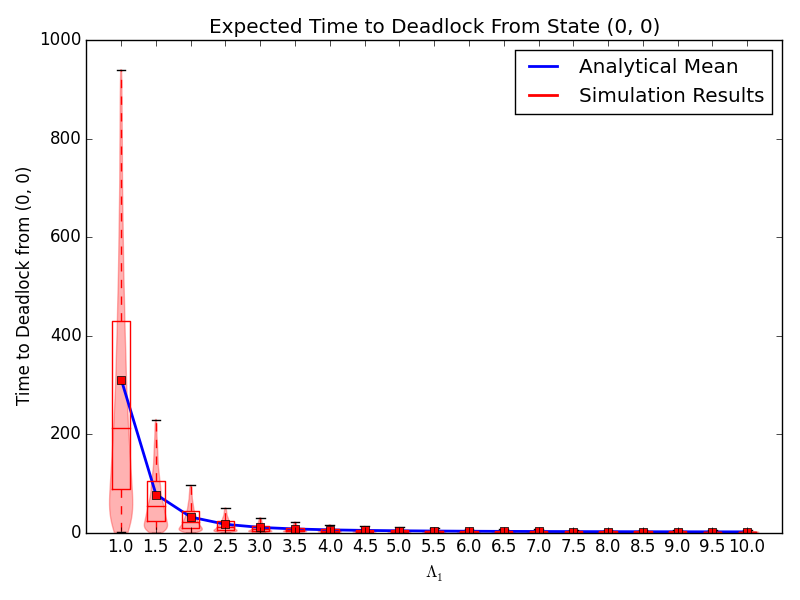
\includegraphics[width=\textwidth]{images/varyL}
  \caption{Varying $\Lambda$}
  \label{fig:timestodeadlock_L}
\end{subfigure}
\begin{subfigure}[b]{0.5\textwidth}
  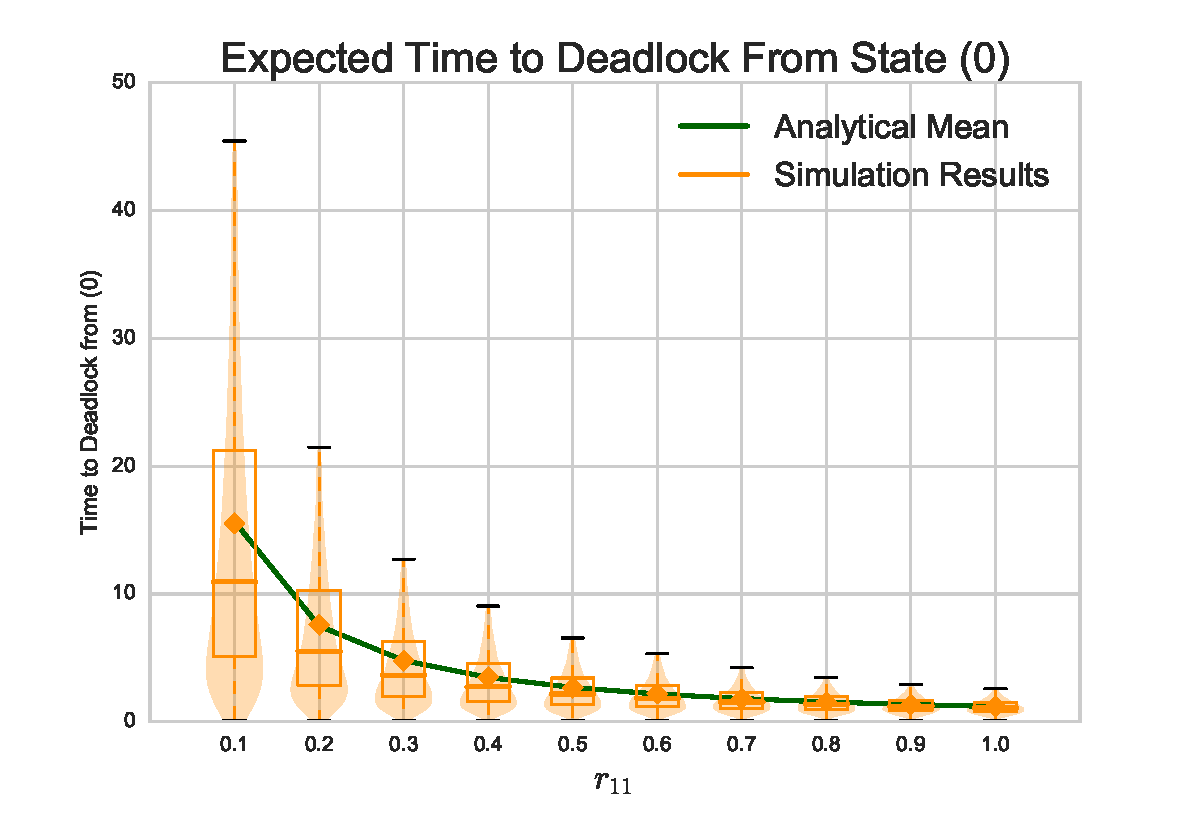
\includegraphics[width=\textwidth]{images/varyr11}
  \caption{Varying $r_{11}$}
  \label{fig:timestodeadlock_r11}
\end{subfigure}
\begin{subfigure}[b]{0.5\textwidth}
  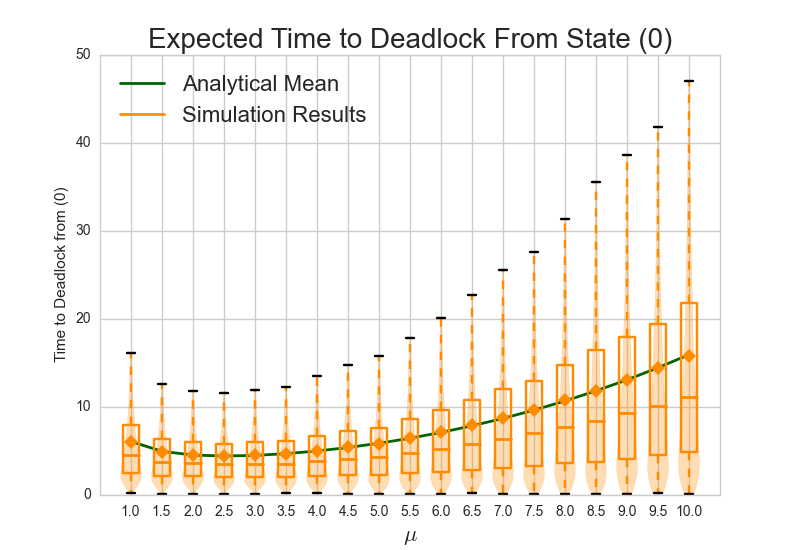
\includegraphics[width=\textwidth]{images/varymu}
  \caption{Varying $\mu$}
  \label{fig:timestodeadlock_mu}
\end{subfigure}
\begin{subfigure}[b]{0.5\textwidth}
  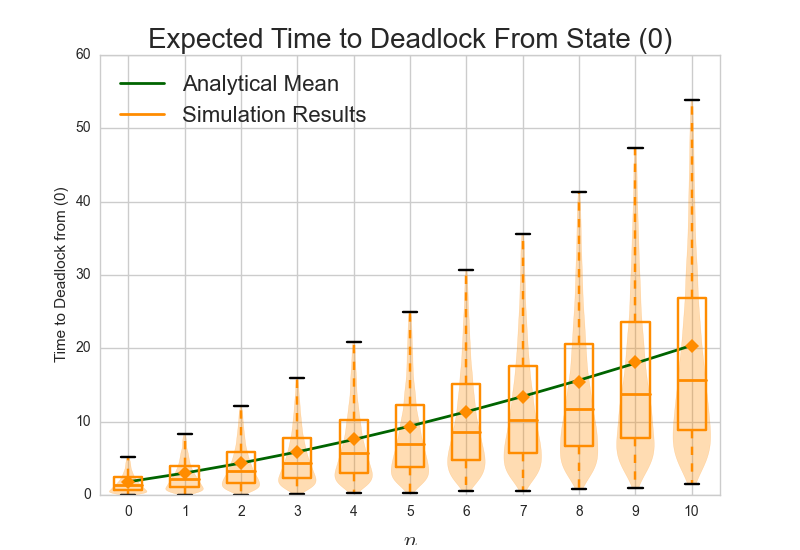
\includegraphics[width=\textwidth]{images/varyn}
  \caption{Varying $n$}
  \label{fig:timestodeadlock_n}
\end{subfigure}
\caption{Time to deadlock in $\Omega_1$, analytical \& simulation results (10,000 iterations).}
\label{fig:timestodeadlock}
\end{figure}

The behaviour as the service rate $\mu$ varies is not monotonic, as the service rate contributed towards both moving customers from the system and allowing customers to rejoin the queue, causing blockages and deadlock.
This behaviour is described in the following lemma.\\

\begin{lemma}\label{lem:oneminima}
The function $\omega_1(\mu)$ that describes the time to deadlock of an $\Omega_1$ system as the service rate $\mu$ varies, and all other parameters are fixed, has one critical point and is a local minimum for $\mu \in (0, \infty)$.
\end{lemma}

\begin{proof}

This proof is by interpretation.
The behaviour of $\omega_1(\mu)$ can be interpreted as follows:
\begin{itemize}
\item At $\lim_{\mu \to 0} \omega_1 (\mu)$ there is infinite service time, and so infinite time until deadlock.
\item At $\lim_{\mu \to \infty} \omega_1 (\mu)$ there is zero service time, the queue can never fill up, and so infinite time to deadlock.
\item At low service rates below a certain threshold $\hat{\mu}$, the arrival rate is relatively large compared to the service rate, and we can assume a saturated system.
At this point services where a customer exits the system does not have much of an effect, as we can assume another arrival immediately.
However services where a customer wishes to rejoin the queue results in a blockage as the system is saturated.
Therefore, increasing the service rate here increases the chance of a blockage, and so the chance of deadlock.
\item Above $\hat{\mu}$ the service rate is large enough that we cannot assume a saturated system, and so services where the customer exits the system does have an affect on the number of customers in the system.
Thus increasing the service rate removes people from the system, and as such there is less chance of getting blocked and deadlocked.
\end{itemize}

\end{proof}

This effect is closely related to the transition rate $r_{11}$, as the rate at which the system enters deadlock from a full queue is $r_{11}\mu$.
Figure~\ref{fig:varymuandr} shows the effect of the transition rate on the behaviour of varying the service rate.

Figures~\ref{fig:threshold_r11}, \ref{fig:threshold_L} and \ref{fig:threshold_n} show the effect of varying $r_{11}$, $\Lambda$ and $n$ on this threshold $\hat{\mu}$ respectively.
In Figure~\ref{fig:threshold_n} it is shown that increasing the queueing capacity lowers the threshold; this is due to the system becoming saturated easier at lower queueing capacities and therefore requiring a larger service rate to escape this saturated zone.
In Figure~\ref{fig:threshold_r11} it is shown that increasing the rejoining probability raises the threshold.
Lower rejoining probabilities make the system escape the saturated zone quicker, and only a low service rate is required to escape; however at high rejoin probabilities a higher service rate fills the system up quicker, and so an even higher service rate is required to escape the saturated zone.
Figure~\ref{fig:threshold_L} implies a positive linear relationship between the arrival rate and the threshold.
Again, at lower arrival rates the system does not fill up as easily, and so is easier to escape the saturated zone.\\

\begin{figure}[!htbp]
  \begin{subfigure}[b]{0.5\textwidth}
    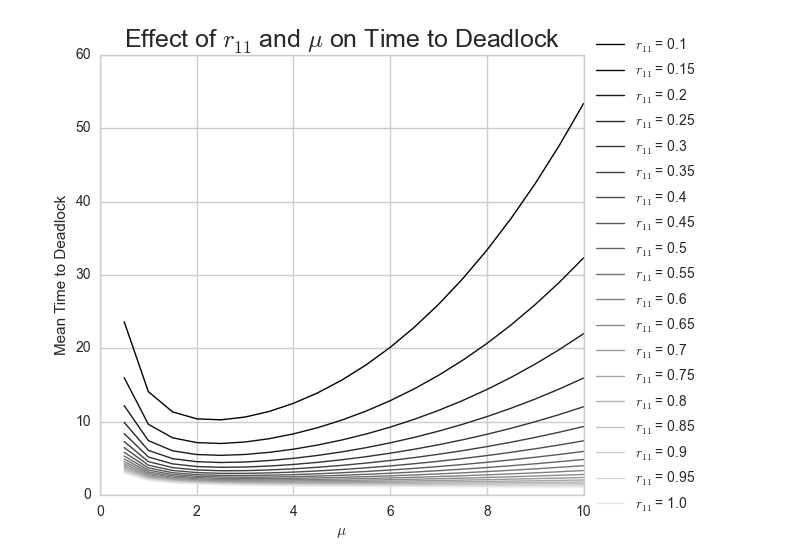
\includegraphics[width=\textwidth]{images/varymur11}
    \caption{The effect of $r_{11}$ and $\mu$ on times to deadlock.}
    \label{fig:varymuandr}
  \end{subfigure}
  \begin{subfigure}[b]{0.5\textwidth}
    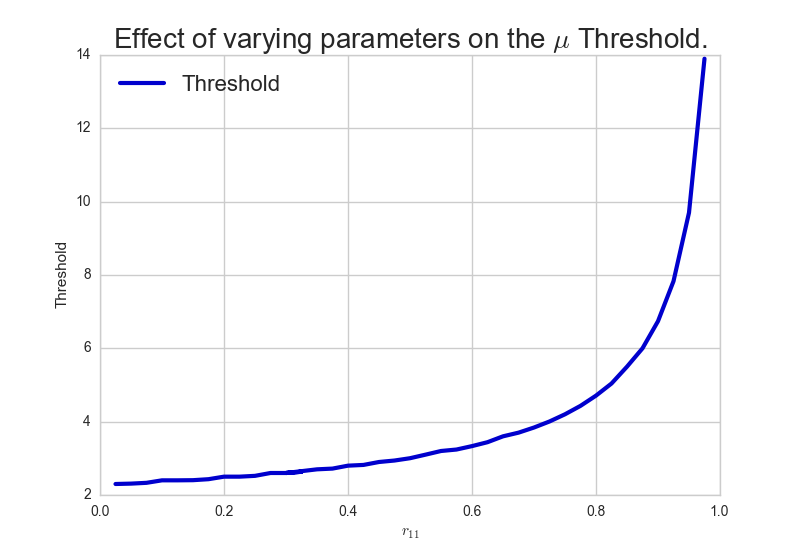
\includegraphics[width=\textwidth]{images/plot_thresholds_r11}
    \caption{The effect of $r_{11}$ on $\hat{\mu}$.}
    \label{fig:threshold_r11}
  \end{subfigure}
  \begin{subfigure}[b]{0.5\textwidth}
    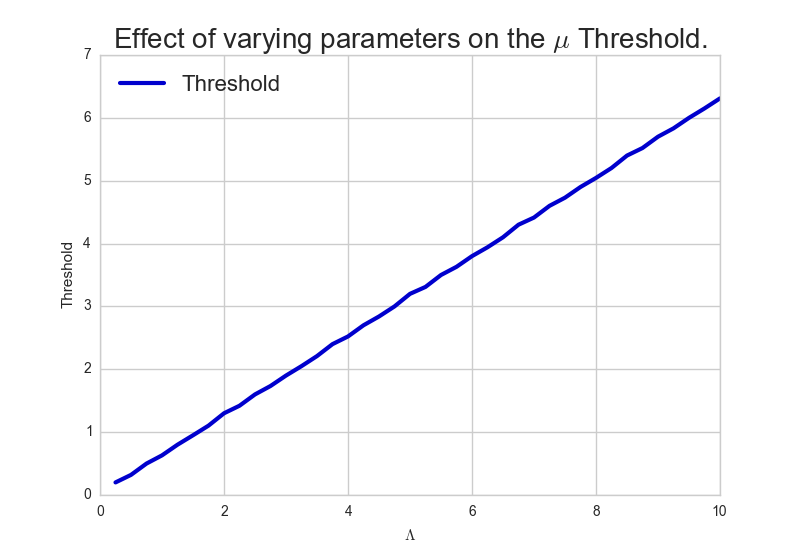
\includegraphics[width=\textwidth]{images/plot_thresholds_L}
    \caption{The effect of $\Lambda$ on $\hat{\mu}$.}
    \label{fig:threshold_L}
  \end{subfigure}
  \begin{subfigure}[b]{0.5\textwidth}
    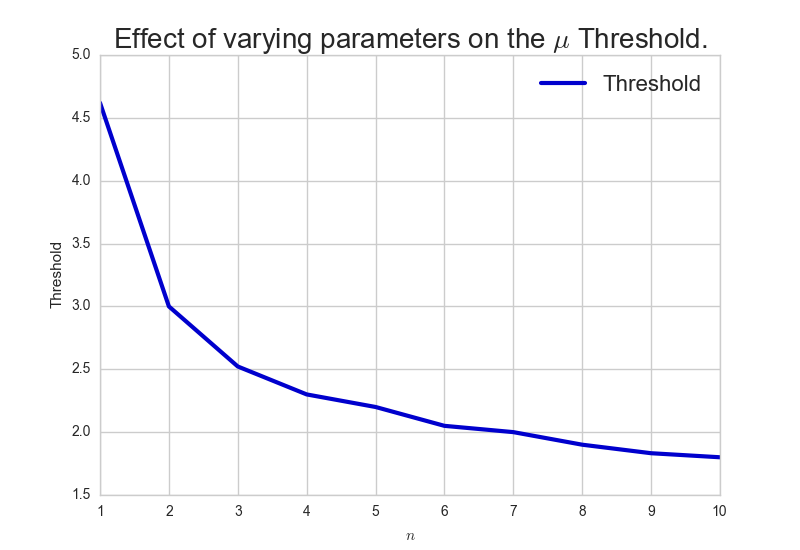
\includegraphics[width=\textwidth]{images/plot_thresholds_n}
    \caption{The effect of $n$ on $\hat{\mu}$.}
    \label{fig:threshold_n}
  \end{subfigure}
  \caption{Investigating the service rate threshold.}
  \label{fig:threshold_investigate}
\end{figure}

\begin{remark}\label{rem:findmaximum}
$\arg\max_{\mu \in [a, b]} \omega_1(\mu)$ is either $a$ or $b$.

From the closed interval method of finding absolute maximum \cite{tan09}, the absolute maximum of $\omega_1(\mu)$ on the closed interal $[a, b]$ is either the critical points in $(a, b)$, $a$ or $b$.
The critical points in $(a, b)$ is $\hat{\mu}$, and is a local minimum (from Lemma~\ref{lem:oneminima}), and so $\hat{\mu} \leq a$ and $\hat{\mu} \leq b$.
Therefore $\omega_1(\mu)$ obtains its maximum at either $a$ or $b$.
\end{remark}

\subsection{Two Node Network without Self Loops}\label{sec:2nodewithoutselfloops}
Consider the queueing network shown in Figure~\ref{fig:queueingnetwork_2nodes}.
This shows two \(M/M/1\) queues, with \(n_i\) queueing capacity at at each service station and service rates $\mu_i$.
$\Lambda_i$ is the external arrival rates to each service station.
All routing possibilities except self loops are possible, where the routing probability from node $i$ to node $j$ is denoted by $r_{ij}$.

Let this system be denoted by $\Omega_2$ with parameter set $(\Lambda_1$, $\Lambda_2$, $\mu_1$, $\mu_2$, $n_1$, $n_2$, $r_{12}$, $r_{21})$.

\begin{figure}[!htbp]
  \includestandalone[width=\textwidth]{images/2nodeexample}
  \caption{A two node queueing network.}
  \label{fig:queueingnetwork_2nodes}
\end{figure}

\begin{itemize}
    \item State space:
        \[S = \{(i,j)\in\mathbb{N}^{(n_1+2\times n_2+2)} \nonscript\; | \nonscript\; 0 \leq i + j \leq n_1 + n_2 + 2
        \}\cup\{(-1)\}\]

        where \(i\) denotes the number of individuals:
            \begin{itemize}
                \item In service or waiting at the first node.
                \item Occupying a server but having finished service at the
                    second node waiting to join the first.
            \end{itemize}
        where \(j\) denotes the number of individuals:
            \begin{itemize}
                \item In service or waiting at the second node.
                \item Occupying a server but having finished service at the
                    first node waiting to join the second.
            \end{itemize}
        and the state $(-1)$ denotes the deadlocked state.
\end{itemize}

If we define $\delta = (i_2, j_2) - (i_1, j_1)$ for all $(i_k, j_k) \in S$, then the transitions are given by:

\begin{equation}
  q_{(i_1, j_1),(i_2, j_2)} = \left\{
  \begin{matrix*}[ r ]
    \left. \begin{matrix*}[ r ]
      \Lambda_1 & \text{if } i_1 < n_1 + 1 \\
      0 & \text{otherwise}
    \end{matrix*} \right\} & \text{if } \delta = (1, 0) \\
    \left. \begin{matrix*}[ r ]
      \Lambda_2 & \text{if } j_1 < n_2 + 1 \\
      0 & \text{otherwise}
    \end{matrix*} \right\} & \text{if } \delta = (0, 1) \\
    \left. \begin{matrix*}[ r ]
      (1 - r_{12})\mu_1 & \text{if } j_1 < n_2 + 2 \\
      0 & \text{otherwise}
    \end{matrix*} \right\} & \text{if } \delta = (-1, 0) \\
    \left. \begin{matrix*}[ r ]
      (1 - r_{21})\mu_2 & \text{if } i_1 < n_1 + 2 \\
      0 & \text{otherwise}
    \end{matrix*} \right\} & \text{if } \delta = (0, -1) \\
    \left. \begin{matrix*}[ r ]
      r_{12}\mu_1 & \text{if } j_1 < n_2 + 2 \text{ and } (i_1, j_1) \neq (n_1 + 2, n_2) \\
      0 & \text{otherwise}
    \end{matrix*} \right\} & \text{if } \delta = (-1, 1) \\
    \left. \begin{matrix*}[ r ]
      r_{21}\mu_2 & \text{if } i_1 < n_1 + 2 \text{ and } (i_1, j_1) \neq (n_1, n_2 + 2) \\
      0 & \text{otherwise}
    \end{matrix*} \right\} & \text{if } \delta = (1, -1) \\
    0 & \text{otherwise}
  \end{matrix*} \right.
\end{equation}

\begin{equation}
  q_{(i_1, j_1), (-1)} = \left\{
  \begin{matrix*}[ r ]
    r_{21}\mu_2 & \text{if } (i, j) = (n_1, n_2 + 2) \\
    r_{12}\mu_1 & \text{if } (i, j) = (n_1 + 2, n_2) \\
    0 & \text{otherwise}
  \end{matrix*}
  \right.
\end{equation}

and

\begin{equation}
  q_{-1, s} = 0
\end{equation}

For $n_1 = 1$ and $n_2 = 2$, the resulting Markov chain is shown in Figure~\ref{fig:2nodeMC}.

\begin{figure}[!htbp]
    \includestandalone[width=\textwidth]{images/markov_chain}
    \caption{Diagrammatic representation of the Markov chain for $\Omega_2$ with $n_1=1$ and $n_2=2$.}
    \label{fig:2nodeMC}
\end{figure}

Figure~\ref{fig:timestodeadlock2} shows the effect of varying the parameters of the above Markov model.
Base parameters of $\Lambda_1 = 4$, $\Lambda_2 = 5$, $n_1 = 3$, $n_2 = 2$, $\mu_1 = 10$, $\mu_2 = 8$, $r_{12} = 0.25$ and $r_{21} = 0.15$ were used.
similar behaviour to Figure~\ref{fig:timestodeadlock} can be seen.

\begin{center}
\begin{figure}[!htbp]
\begin{center}
\begin{subfigure}[b]{0.38\textwidth}
  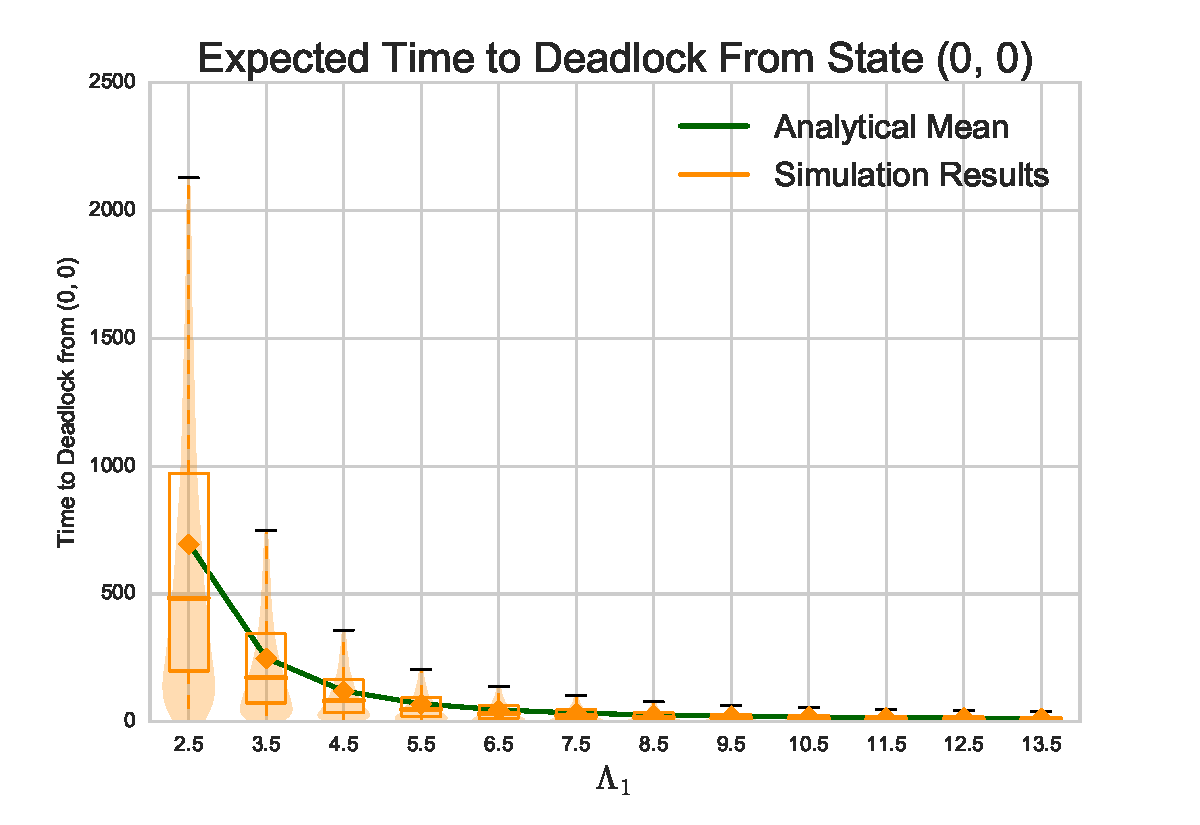
\includegraphics[width=\textwidth]{images/varyL1}
  \caption{Varying $\Lambda_1$}
  \label{fig:timestodeadlock2_L1}
\end{subfigure}
\begin{subfigure}[b]{0.38\textwidth}
  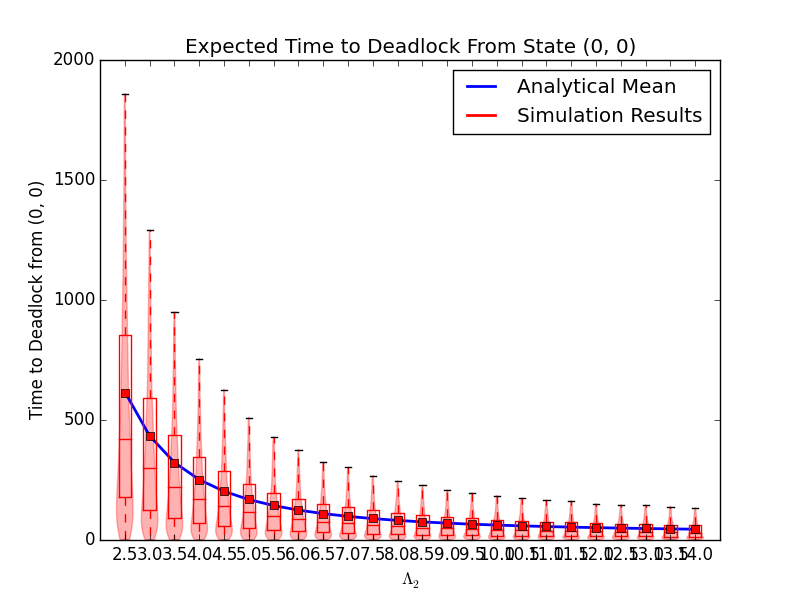
\includegraphics[width=\textwidth]{images/varyL2}
  \caption{Varying $\Lambda_2$}
  \label{fig:timestodeadlock2_L2}
\end{subfigure}
\begin{subfigure}[b]{0.38\textwidth}
  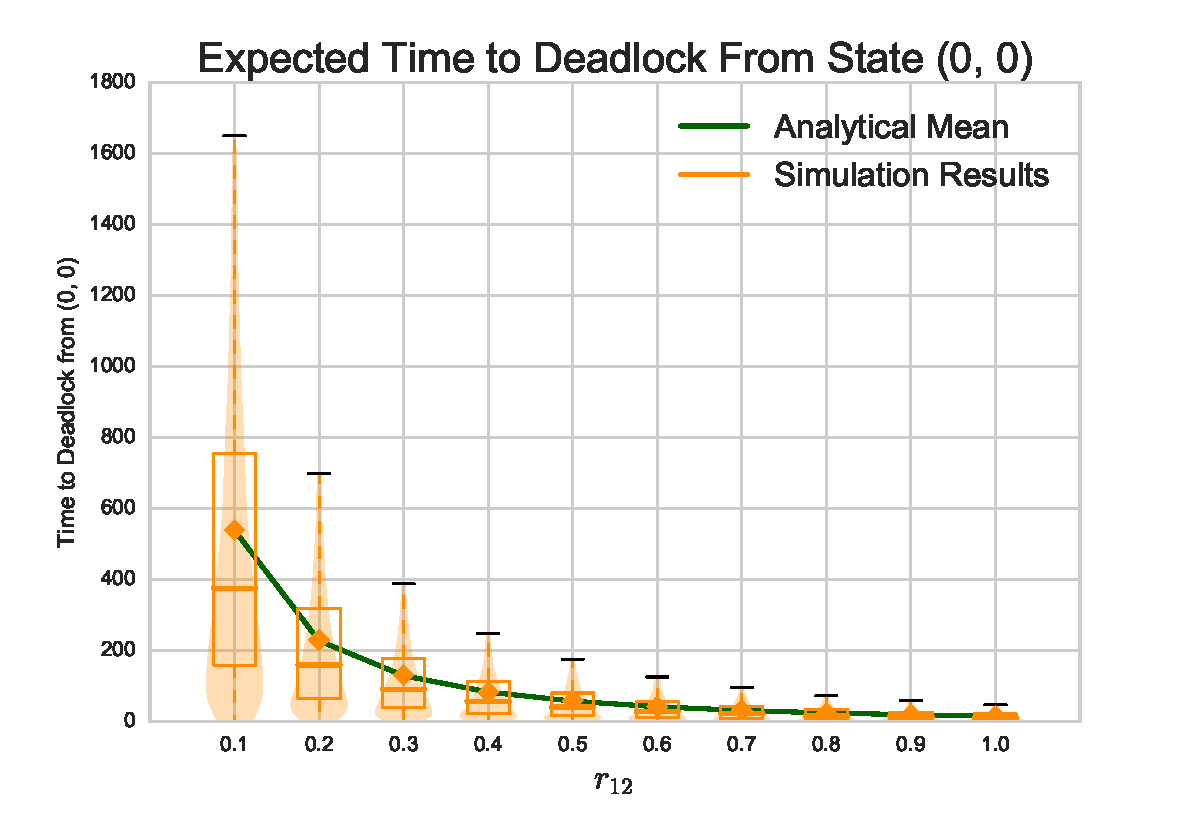
\includegraphics[width=\textwidth]{images/varyr12}
  \caption{Varying $r_{12}$}
  \label{fig:timestodeadlock2_r12}
\end{subfigure}
\begin{subfigure}[b]{0.38\textwidth}
  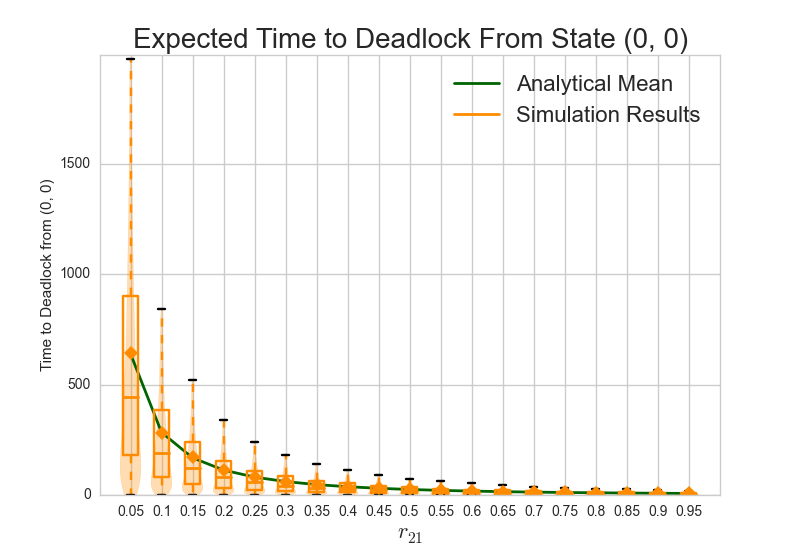
\includegraphics[width=\textwidth]{images/varyr21}
  \caption{Varying $r_{21}$}
  \label{fig:timestodeadlock2_r21}
\end{subfigure}
\begin{subfigure}[b]{0.38\textwidth}
  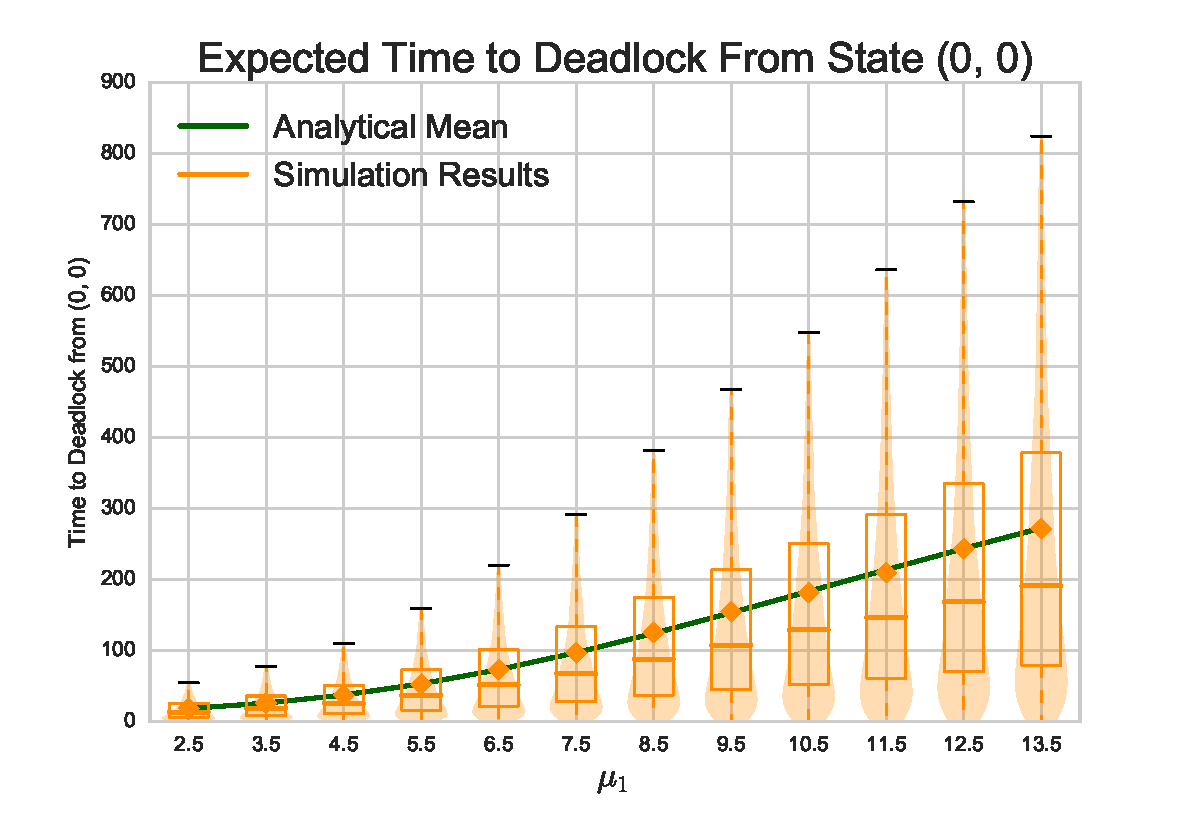
\includegraphics[width=\textwidth]{images/varymu1}
  \caption{Varying $\mu_1$}
  \label{fig:timestodeadlock2_mu1}
\end{subfigure}
\begin{subfigure}[b]{0.38\textwidth}
  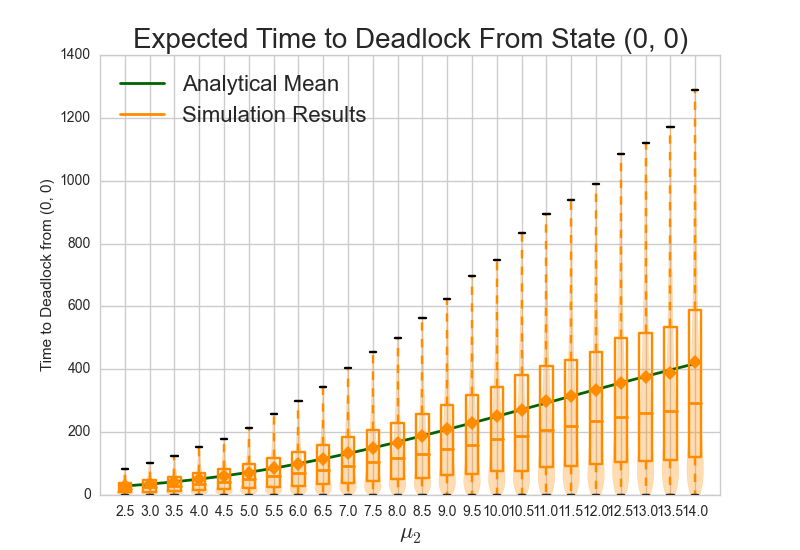
\includegraphics[width=\textwidth]{images/varymu2}
  \caption{Varying $\mu_2$}
  \label{fig:timestodeadlock2_mu2}
\end{subfigure}
\begin{subfigure}[b]{0.38\textwidth}
  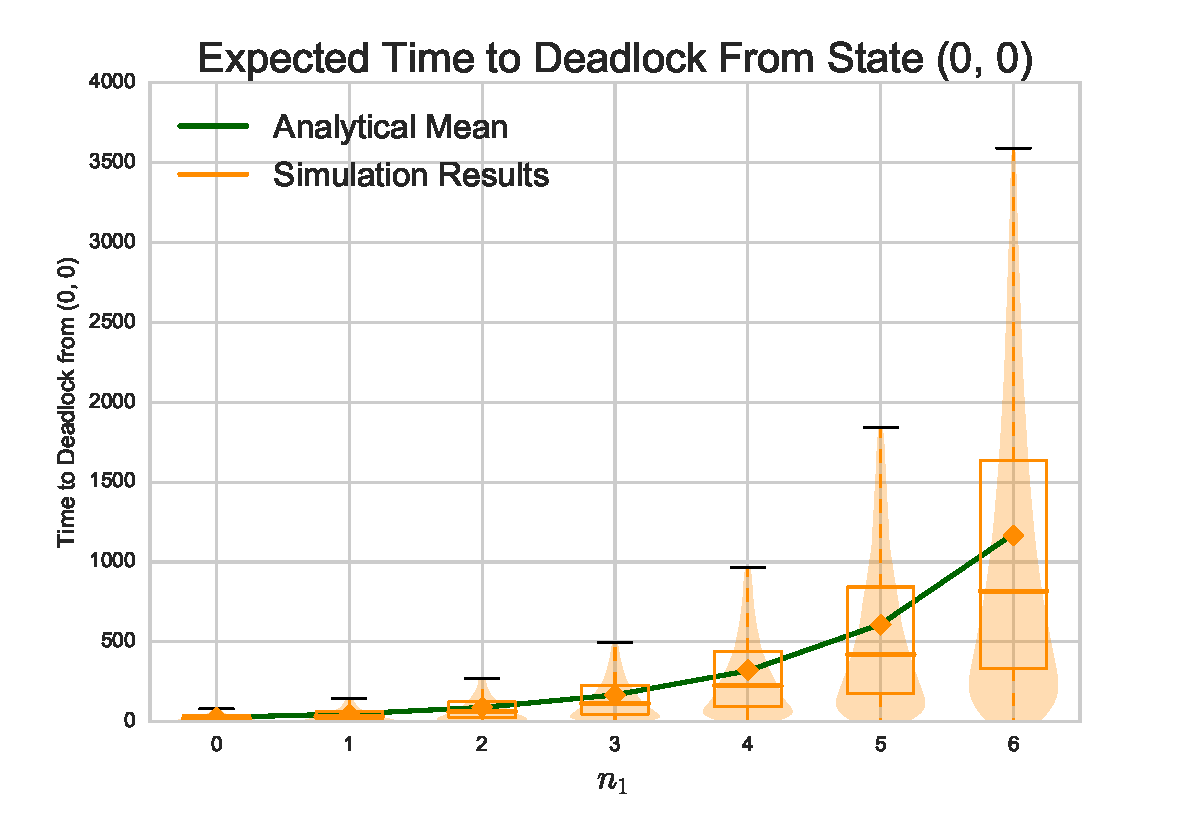
\includegraphics[width=\textwidth]{images/varyn1}
  \caption{Varying $n_1$}
  \label{fig:timestodeadlock2_n1}
\end{subfigure}
\begin{subfigure}[b]{0.38\textwidth}
  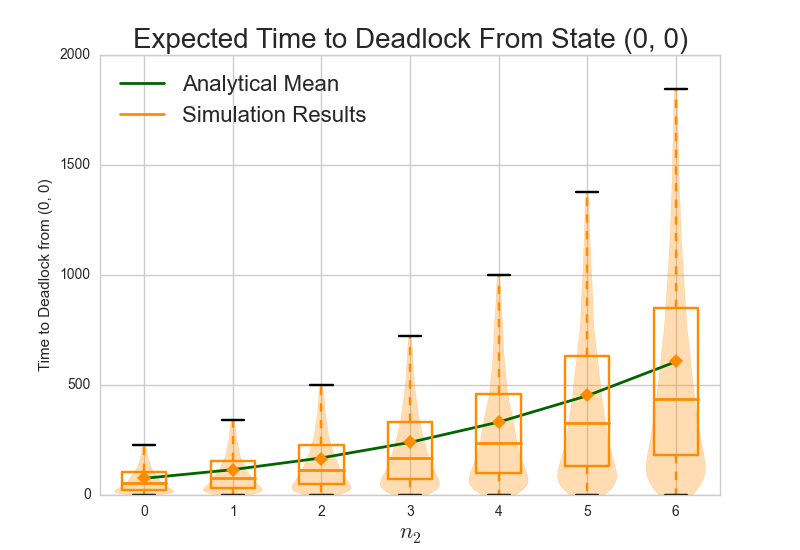
\includegraphics[width=\textwidth]{images/varyn2}
  \caption{Varying $n_2$}
  \label{fig:timestodeadlock2_n2}
\end{subfigure}
\end{center}
\caption{Time to deadlock in $\Omega_2$, analytical \& simulation results (10,000 iterations).}
\label{fig:timestodeadlock2}
\end{figure}
\end{center}


\subsection{Complete Two Node Network}\label{sec:2nodeselfloops}
Consider the queueing network shown in Figure~\ref{fig:queueingnetwork_2nodesfeedback}.
This shows two \(M/M/1\) queues, with \(n_i\) queueing capacity at at each service station and service rates $\mu_i$.
$\Lambda_i$ is the external arrival rates to each service station.
All routing possibilities are possible, where the routing probability from node $i$ to node $j$ is denoted by $r_{ij}$.

Let this system be denoted by $\Omega$ with parameter set $(\Lambda_1$, $\Lambda_2$, $\mu_1$, $\mu_2$, $n_1$, $n_2$, $r_{11}$, $r_{12}$, $r_{21}$, $r_{22})$.

\begin{figure}[!htbp]
  \includestandalone[width=\textwidth]{images/2nodefeedbackexample}
  \caption{A complete two node queueing network.}
  \label{fig:queueingnetwork_2nodesfeedback}
\end{figure}

\begin{itemize}
    \item State space:
        \[S = \{(i,j)\in\mathbb{N}^{(n_1+2\times n_2+2)} \nonscript\; | \nonscript\; 0 \leq i + j \leq n_1 + n_2 + 2
        \}\cup\{(-1), (-2), (-3)\}\]

        where \(i\) denotes the number of individuals:
            \begin{itemize}
                \item In service or waiting at the first node.
                \item Occupying a server but having finished service at the
                    second node waiting to join the first.
            \end{itemize}
        where \(j\) denotes the number of individuals:
            \begin{itemize}
                \item In service or waiting at the second node.
                \item Occupying a server but having finished service at the
                    first node waiting to join the second.
            \end{itemize}
        and the state $(-3)$ denotes the deadlocked state cause by both nodes; $(-1)$ denotes the deadlocked state caused by the first node only; and $(-2)$ denotes the deadlocked state caused by the second node only. (Recall the different configurations of deadlock in Figure~\ref{fig:4nodecombinations})
\end{itemize}

If we define $\delta = (i_2, j_2) - (i_1, j_1)$ for all $(i_k, j_k) \in S$, then the transitions are given by:

\begin{equation}
  q_{(i_1, j_1),(i_2, j_2)} = \left\{
  \begin{matrix*}[ r ]
    \left. \begin{matrix*}[ r ]
      \Lambda_1 & \text{if } i_1 < n_1 + 1 \\
      0 & \text{otherwise}
    \end{matrix*} \right\} & \text{if } \delta = (1, 0) \\
    \left. \begin{matrix*}[ r ]
      \Lambda_2 & \text{if } j_1 < n_2 + 1 \\
      0 & \text{otherwise}
    \end{matrix*} \right\} & \text{if } \delta = (0, 1) \\
    \left. \begin{matrix*}[ r ]
      (1 - r_{11} - r_{12})\mu_1 & \text{if } j_1 < n_2 + 2 \\
      0 & \text{otherwise}
    \end{matrix*} \right\} & \text{if } \delta = (-1, 0) \\
    \left. \begin{matrix*}[ r ]
      (1 - r_{21} - r_{22})\mu_2 & \text{if } i_1 < n_1 + 2 \\
      0 & \text{otherwise}
    \end{matrix*} \right\} & \text{if } \delta = (0, -1) \\
    \left. \begin{matrix*}[ r ]
      r_{12}\mu_1 & \text{if } j_1 < n_2 + 2 \text{ and } (i_1, j_1) \neq (n_1 + 2, n_2) \\
      0 & \text{otherwise}
    \end{matrix*} \right\} & \text{if } \delta = (-1, 1) \\
    \left. \begin{matrix*}[ r ]
      r_{21}\mu_2 & \text{if } i_1 < n_1 + 2 \text{ and } (i_1, j_1) \neq (n_1, n_2 + 2) \\
      0 & \text{otherwise}
    \end{matrix*} \right\} & \text{if } \delta = (1, -1) \\
    0 & \text{otherwise}
  \end{matrix*} \right.
\end{equation}

\begin{equation}\label{equ:todeadlock2}
  q_{(i_1, j_1), (-1)} = \left\{
  \begin{matrix*}[ r ]
    r_{11}\mu_1 & \text{if } i > n_1 \text{ and } j < n_2 + 2 \\
    0 & \text{otherwise}
  \end{matrix*}
  \right.
\end{equation}

\begin{equation}\label{equ:todeadlock3}
  q_{(i_1, j_1), (-2)} = \left\{
  \begin{matrix*}[ r ]
    r_{22}\mu_2 & \text{if } j > n_2 \text{ and } i < n_1 + 2 \\
    0 & \text{otherwise}
  \end{matrix*}
  \right.
\end{equation}

\begin{equation}
  q_{(i_1, j_1), (-3)} = \left\{
  \begin{matrix*}[ r ]
    r_{21}\mu_2 & \text{if } (i, j) = (n_1, n_2 + 2) \\
    r_{12}\mu_1 & \text{if } (i, j) = (n_1 + 2, n_2) \\
    0 & \text{otherwise}
  \end{matrix*}
  \right.
\end{equation}

and

\begin{align}
  q_{-1, s} = 0 \\
  q_{-2, s} = 0 \\
  q_{-3, s} = 0
\end{align}

Note that the there are only two differences between this formulation and the formulation given in Subsection~\ref{sec:2nodewithoutselfloops}: the probabilities of leaving nodes 1 and 2 are now $(1-r_{11}-r_{12})\mu_1$ and $(1-r_{21}-r_{22})\mu_2$; and there are now two more ways to reach deadlock, Equation~\ref{equ:todeadlock2} and Equation~\ref{equ:todeadlock3}.

For $n_1 = 1$ and $n_2 = 2$, the resulting Markov chain is shown in Figure~\ref{fig:2nodeMCfeedback}.

\begin{figure}[!htbp]
    \includestandalone[width=\textwidth]{images/markov_chain_feedback}
    \caption{Diagrammatic representation of the Markov chain for $\Omega$ with $n_1=1$ and $n_2=2$.}
    \label{fig:2nodeMCfeedback}
\end{figure}

Figure~\ref{fig:timestodeadlockfeedback} shows the effect of varying the parameters of the above Markov model.
Base parameters of $\Lambda_1 = 4$, $\Lambda_2 = 5$, $n_1 = 3$, $n_2 = 2$, $\mu_1 = 10$, $\mu_2 = 8$, $r_{11} = 0.1$, $r_{12} = 0.25$, $r_{21} = 0.15$ and $r_{22} = 0.1$ were used.


\begin{figure}[!htbp]
\begin{subfigure}[b]{0.5\textwidth}
  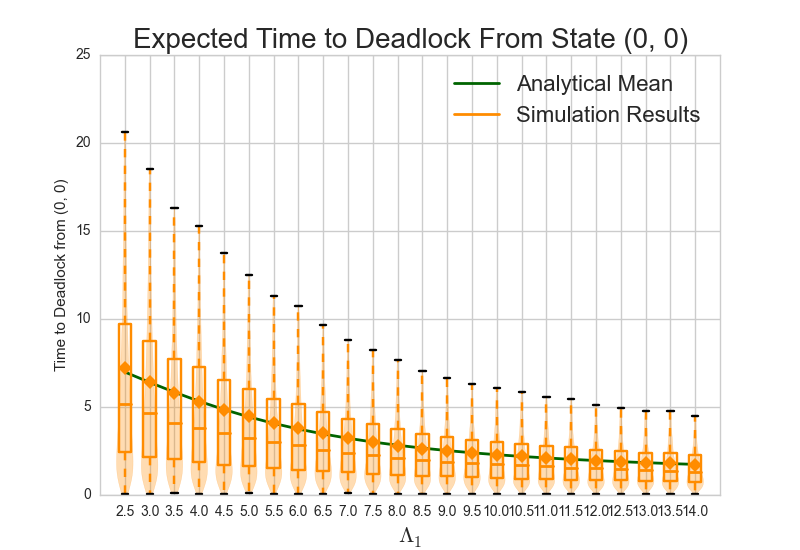
\includegraphics[width=\textwidth]{images/vary_L1fb}
  \caption{Varying $\Lambda_1$}
  \label{fig:timestodeadlockfb_L1}
\end{subfigure}
\begin{subfigure}[b]{0.5\textwidth}
  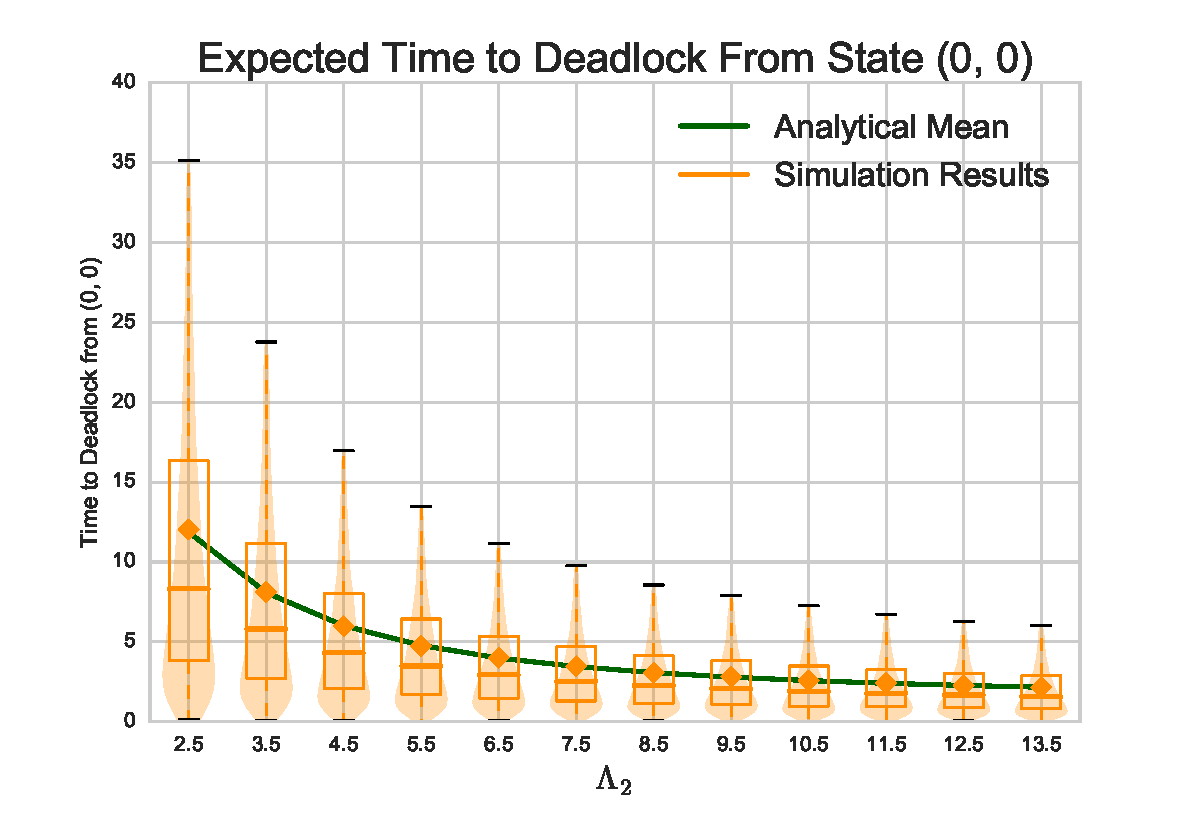
\includegraphics[width=\textwidth]{images/vary_L2fb}
  \caption{Varying $\Lambda_2$}
  \label{fig:timestodeadlockfb_L2}
\end{subfigure}
\begin{subfigure}[b]{0.5\textwidth}
  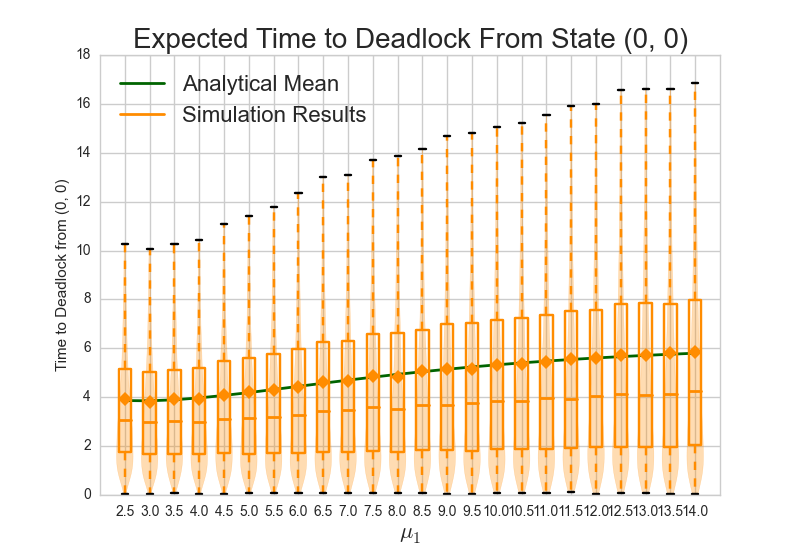
\includegraphics[width=\textwidth]{images/vary_mu1fb}
  \caption{Varying $\mu_1$}
  \label{fig:timestodeadlockfb_mu1}
\end{subfigure}
\begin{subfigure}[b]{0.5\textwidth}
  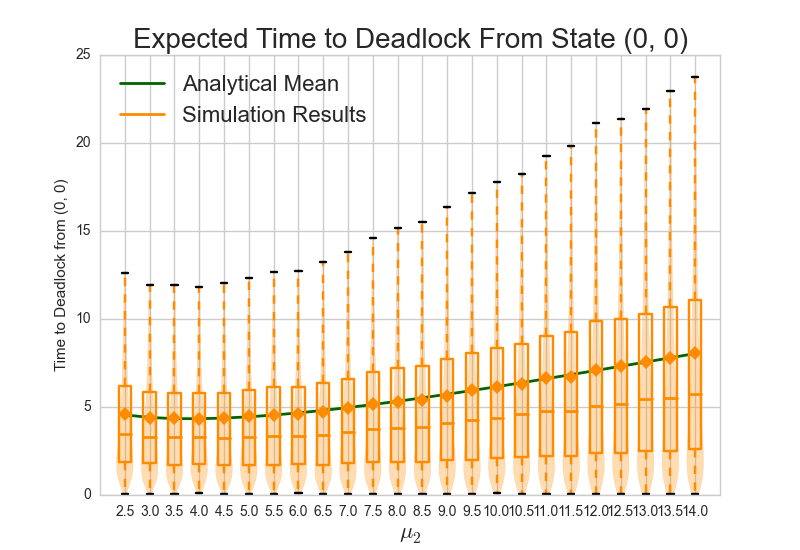
\includegraphics[width=\textwidth]{images/vary_mu2fb}
  \caption{Varying $\mu_2$}
  \label{fig:timestodeadlockfb_mu2}
\end{subfigure}
\begin{subfigure}[b]{0.5\textwidth}
  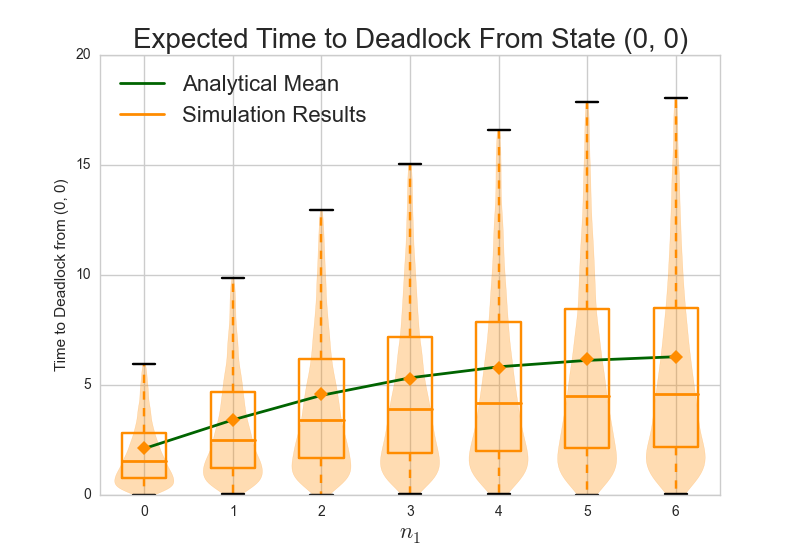
\includegraphics[width=\textwidth]{images/vary_n1fb}
  \caption{Varying $n_1$}
  \label{fig:timestodeadlockfb_n1}
\end{subfigure}
\begin{subfigure}[b]{0.5\textwidth}
  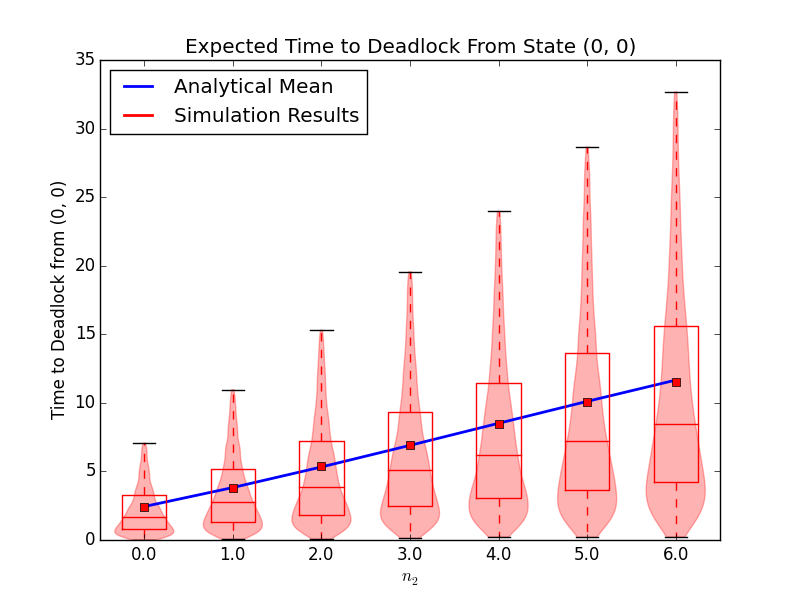
\includegraphics[width=\textwidth]{images/vary_n2fb}
  \caption{Varying $n_2$}
  \label{fig:timestodeadlockfb_n2}
\end{subfigure}
\caption{Time to deadlock in $\Omega$, analytical \& simulation results (10,000 iterations).}
\label{fig:timestodeadlockfeedback}
\end{figure}

The heatmaps in Figure~\ref{fig:heatmaps} illustrate how varying the two transition probabilities out of each node affects the time to deadlock.
Note the shape of the heatmap, this is due to the restriction that $r_{11} + r_{12} \leq 1$ and $r_{21} + r_{22} \leq 1$.
We can see for both nodes it is the rejoining probability ($r_{11}$ and $r_{22}$) that has the most drastic effect on time to deadlock.
This effect is greater for Node 2, the node that has the smaller queueing capacity.

\begin{figure}[!htbp]
\begin{subfigure}[b]{0.5\textwidth}
  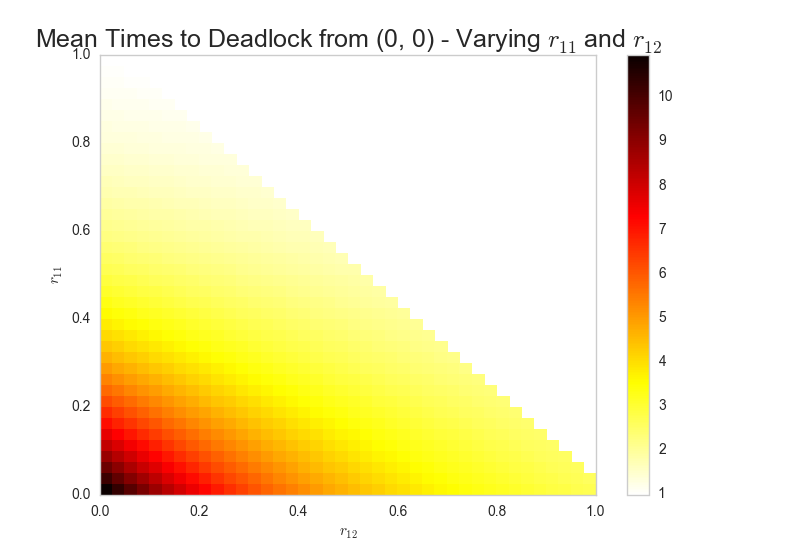
\includegraphics[width=\textwidth]{images/N1_heatmap}
  \caption{Analytical: Varying transition probabilities at Node 1}
  \label{fig:heatmap_anal_1}
\end{subfigure}
\begin{subfigure}[b]{0.5\textwidth}
  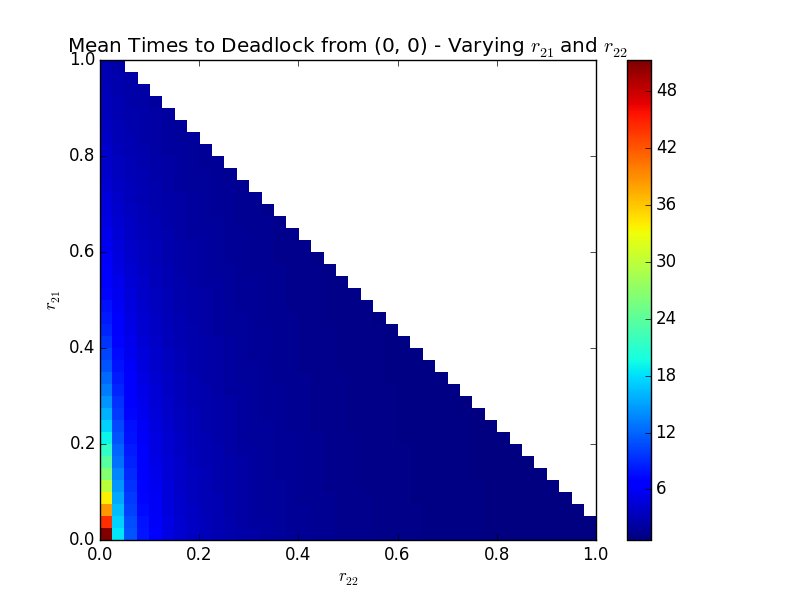
\includegraphics[width=\textwidth]{images/N2_heatmap}
  \caption{Analytical: Varying transition probabilities at Node 2}
  \label{fig:heatmap_anal_2}
\end{subfigure}
\begin{subfigure}[b]{0.5\textwidth}
  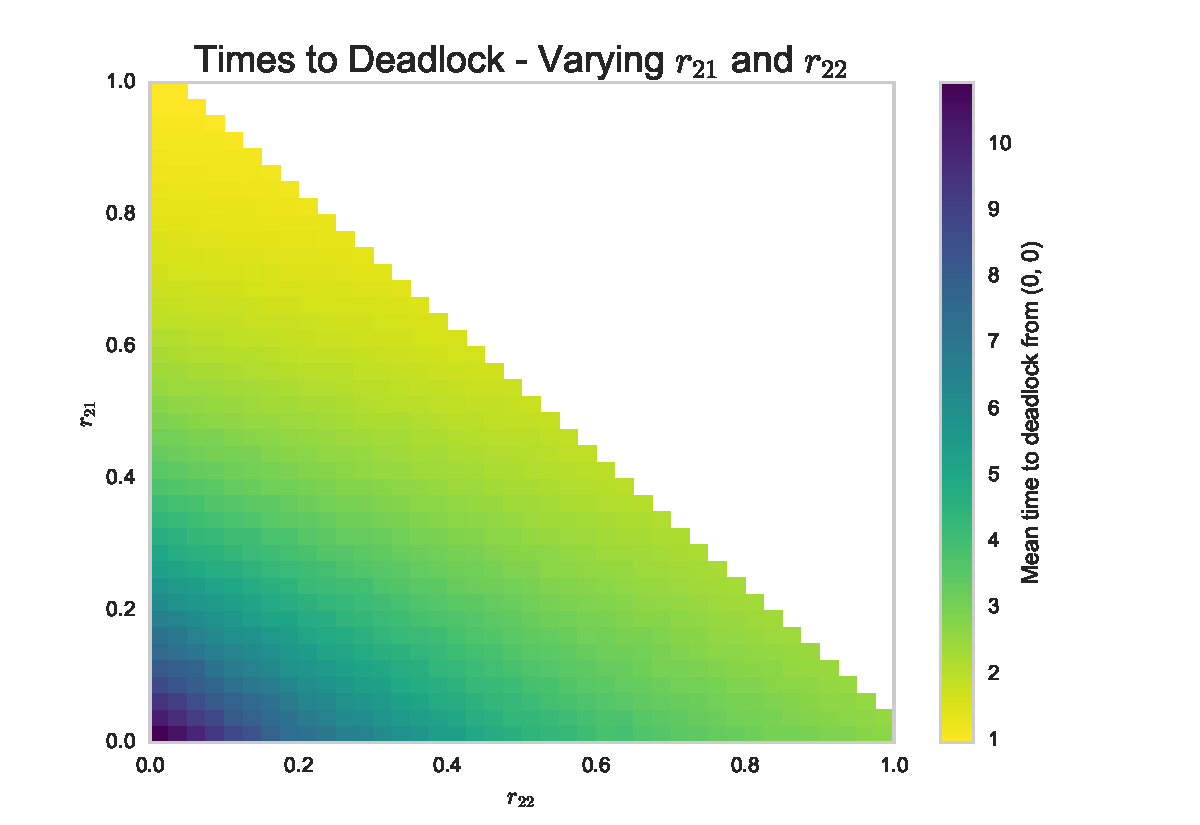
\includegraphics[width=\textwidth]{images/N1_heatmap_sim}
  \caption{Simulation: Varying transition probabilities at Node 1}
  \label{fig:heatmap_sim_1}
\end{subfigure}
\begin{subfigure}[b]{0.5\textwidth}
  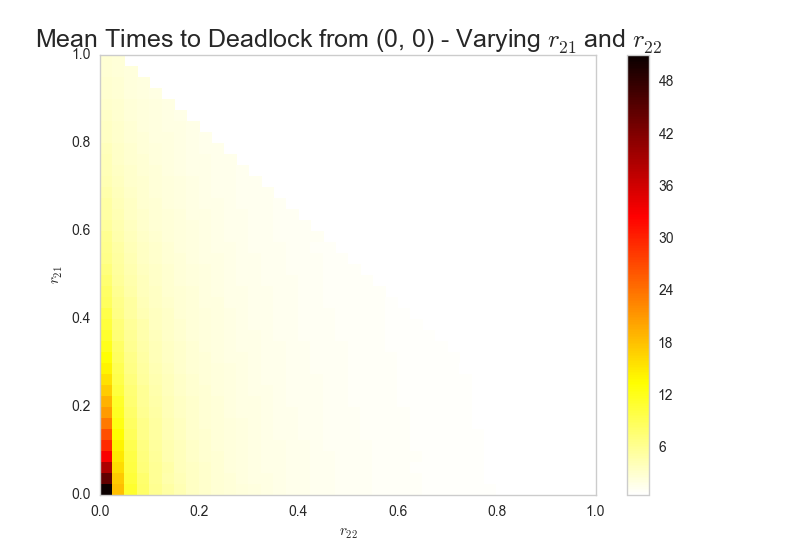
\includegraphics[width=\textwidth]{images/N2_heatmap_sim}
  \caption{Simulation: Varying transition probabilities at Node 2}
  \label{fig:heatmap_sim_2}
\end{subfigure}
\caption{Analytical \& Simulation Results of Times to Deadlock, varying Transition Probabilities (10,000 iterations)}
\label{fig:heatmaps}
\end{figure}

Times to deadlock in this case means the time to the first instance of deadlock.
There is however three different deadlocked states which the queueing network can fall into, (-1), (-2) and (-3).

Figure~\ref{fig:absorbingprobs} shows how varying the parameters of the queueing network affects the absorption probabilities.

\begin{figure}[!htbp]
\begin{subfigure}[b]{0.5\textwidth}
  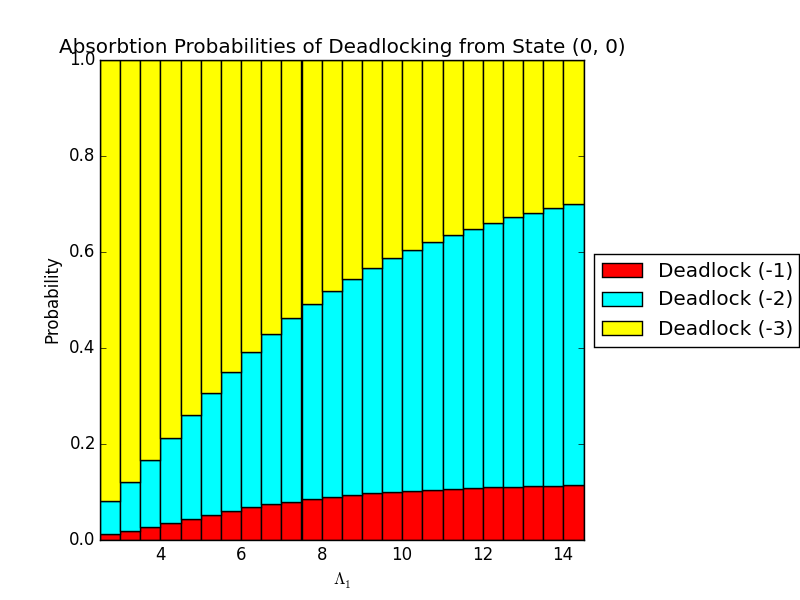
\includegraphics[width=\textwidth]{images/absprobL1}
  \caption{Varying $\Lambda_1$}
  \label{fig:absprobL1}
\end{subfigure}
\begin{subfigure}[b]{0.5\textwidth}
  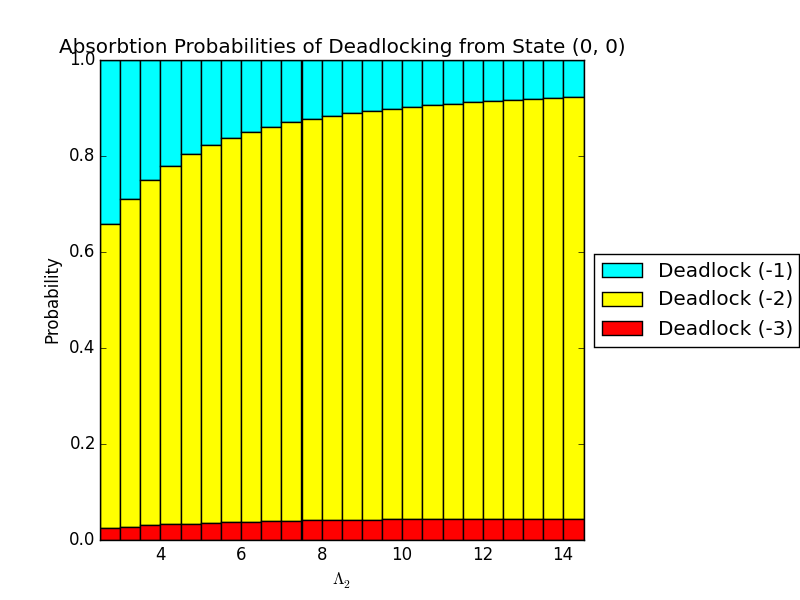
\includegraphics[width=\textwidth]{images/absprobL2}
  \caption{Varying $\Lambda_2$}
  \label{fig:absprobL2}
\end{subfigure}
\begin{subfigure}[b]{0.5\textwidth}
  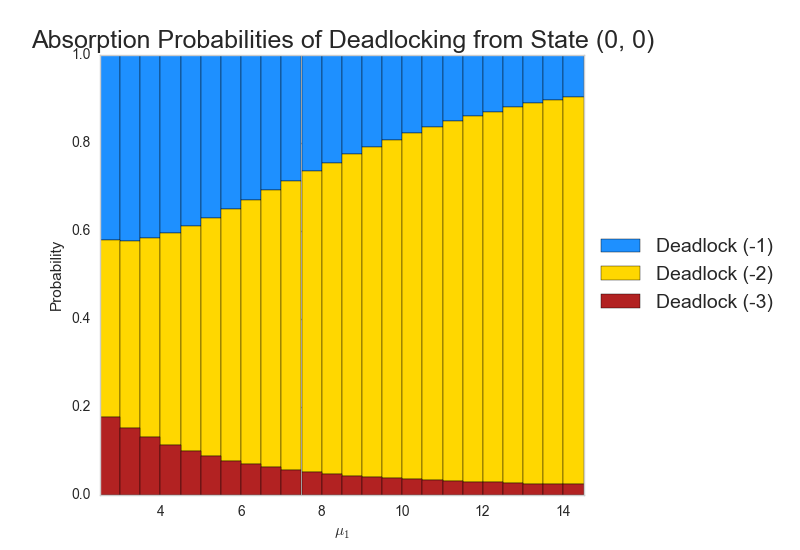
\includegraphics[width=\textwidth]{images/absprobmu1}
  \caption{Varying $\mu_1$}
  \label{fig:absprobmu1}
\end{subfigure}
\begin{subfigure}[b]{0.5\textwidth}
  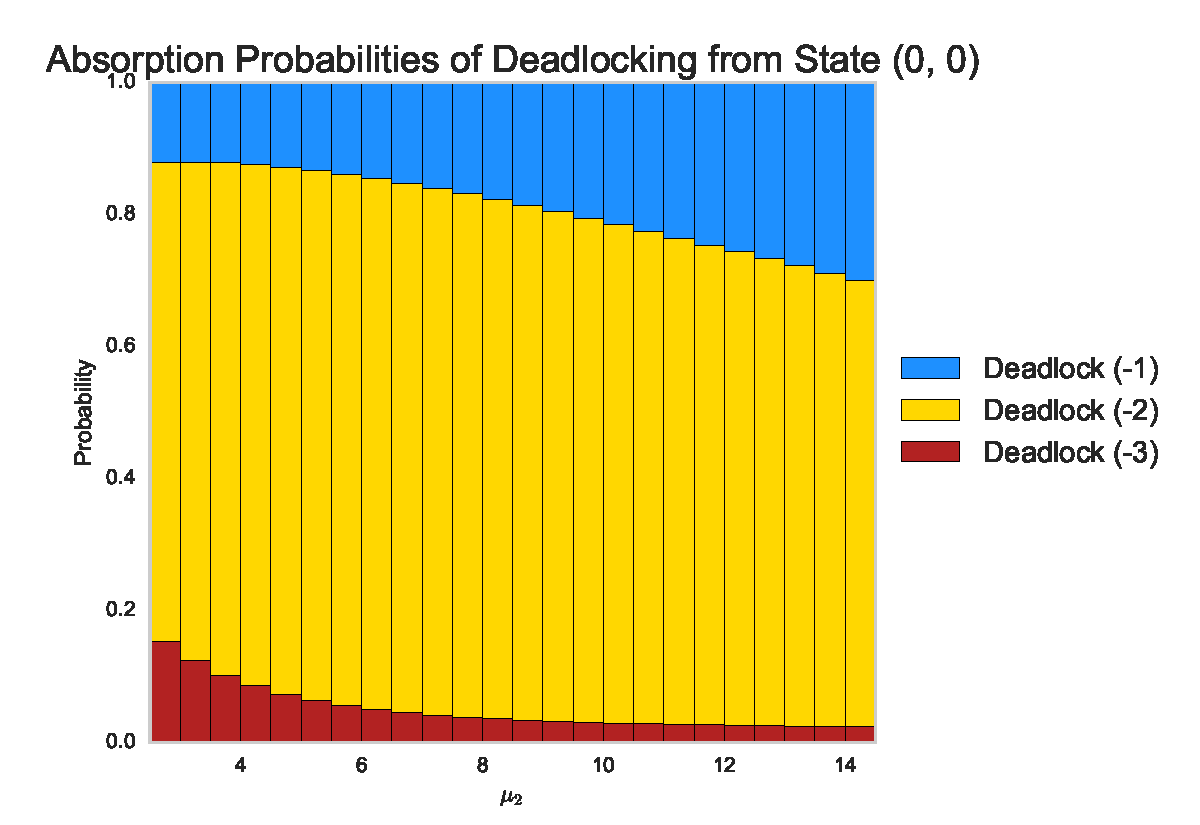
\includegraphics[width=\textwidth]{images/absprobmu2}
  \caption{Varying $\mu_2$}
  \label{fig:absprobmu2}
\end{subfigure}
\begin{subfigure}[b]{0.5\textwidth}
  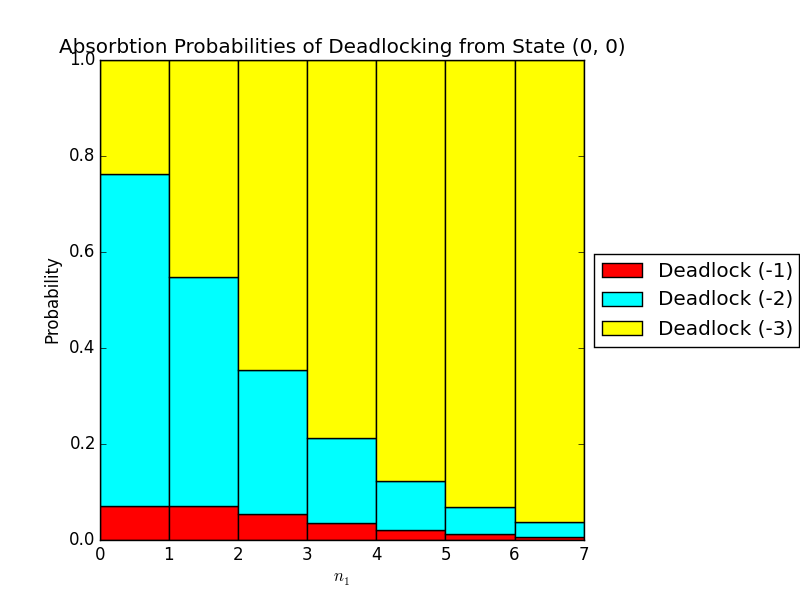
\includegraphics[width=\textwidth]{images/absprobn1}
  \caption{Varying $n_1$}
  \label{fig:absprobn1}
\end{subfigure}
\begin{subfigure}[b]{0.5\textwidth}
  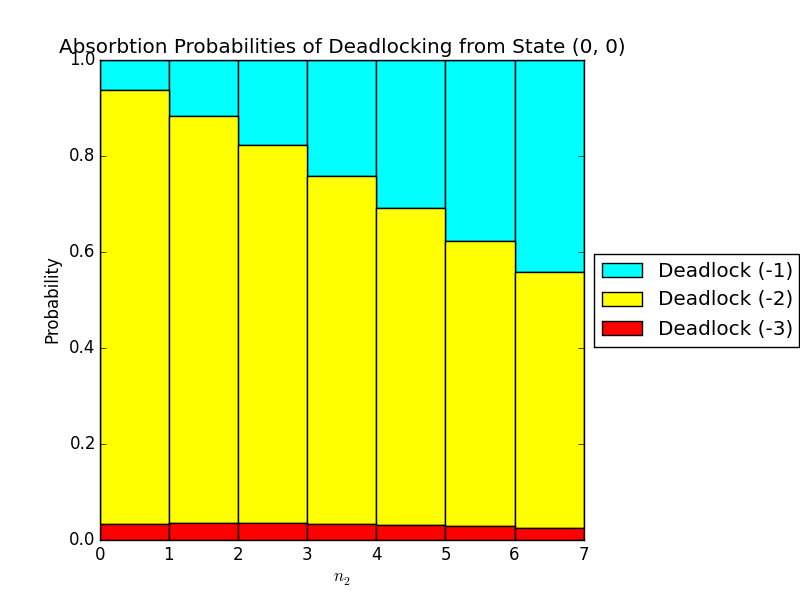
\includegraphics[width=\textwidth]{images/absprobn2}
  \caption{Varying $n_2$}
  \label{fig:absprobn2}
\end{subfigure}
\caption{Probabilities of reaching each deadlocked state.}
\label{fig:absorbingprobs}
\end{figure}

Figure~\ref{fig:timestodeadlockfb_n1} shows that increasing queueing capacity is no longer nearly linear.
Increasing $n_1$ causes a longer time to deadlock up to a point, where increasing $n_1$ any more does not affect the time to deadlock.
This is due to the fact that there are other ways to get to deadlock, and we are only interested in the first instance of any of these deadlocks.
Getting to deadlocked state (-2) is not affected by $n_1$, and so once $n_1$ goes over a certain threshold the system always reaches (-2) before any other deadlocked state, and so the time to deadlock is unaffected by increasing $n_1$ any further.

This behaviour is exhibited as $n_2$ increases too, however this threshold will take longer to reach as the base parameter for $n_1$ is larger than the base parameter for $n_2$.

This behaviour is highlighted in the heatmap shown in Figure~\ref{fig:capacitiesheatmap}, where the analytical mean time to deadlock is shown with combinations of $n_1$ and $n_2$.
For each value of $n_2$, once a certain threshold of $n_1$ is reached no more change in time to deadlock occurs.
Similarly for each value of $n_1$, once a certain threshold o $n_2$ is reached no more change in time to deadlock occurs.
The behaviour is unsymmetrical due to the other parameters associated with Node 1 and Node 2 being unsymmetrical.

\begin{figure}[!htbp]
  \begin{center}
  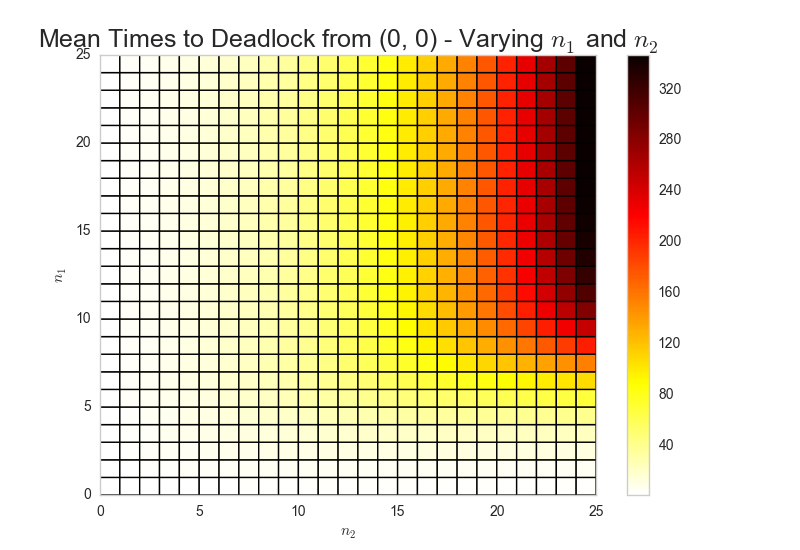
\includegraphics[width=0.5\textwidth]{images/n1n2_heatmap}
  \caption{Deadlocking behaviour, varying $n_1$ and $n_2$}
  \label{fig:capacitiesheatmap}
  \end{center}
\end{figure}

\begin{figure}[!htbp]
  \begin{subfigure}[b]{0.5\textwidth}
    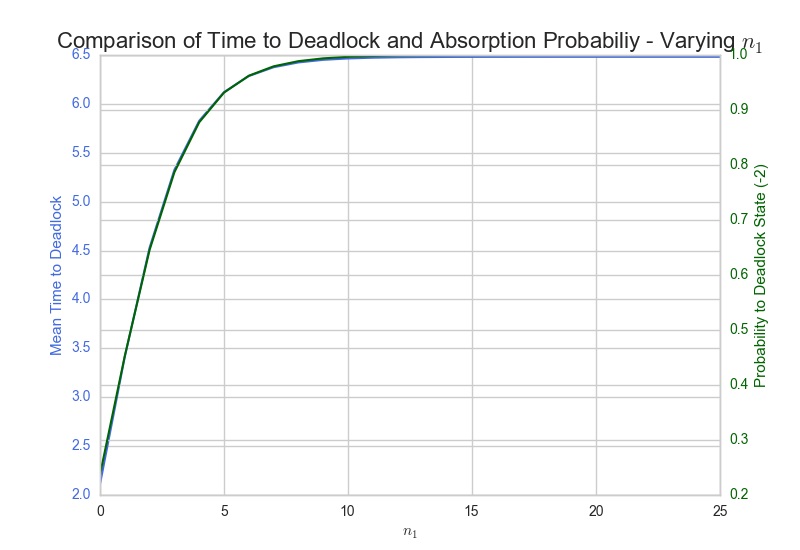
\includegraphics[width=\textwidth]{images/comparetimeprobn1}
    \caption{Varying $n_1$}
    \label{fig:comparetimeprob_n1}
  \end{subfigure}
  \begin{subfigure}[b]{0.5\textwidth}
    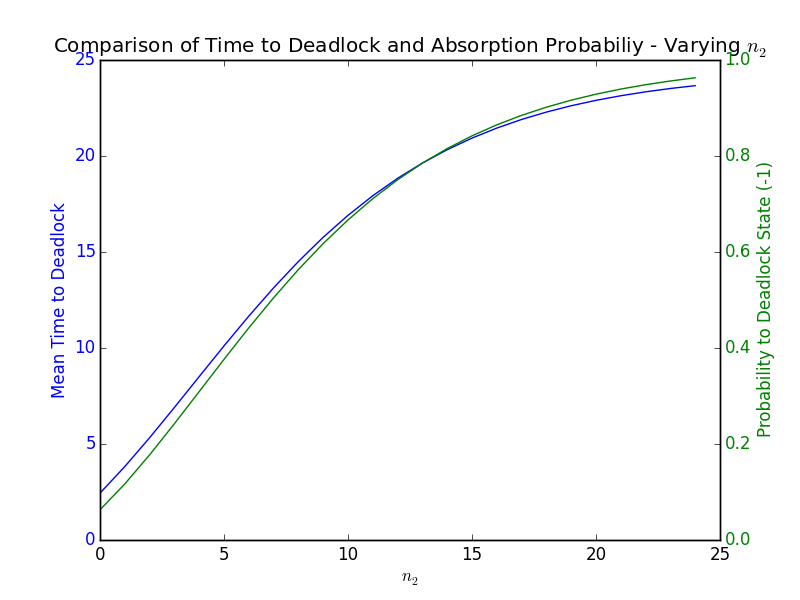
\includegraphics[width=\textwidth]{images/comparetimeprobn2}
    \caption{Varying $n_2$}
    \label{fig:comparetimeprob_n2}
  \end{subfigure}
  \caption{Comparing time to deadlock and absorption probabilities as queue capacities increase.}
  \label{fig:comparetimeprob_ns}
\end{figure}

Figure~\ref{fig:comparetimeprob_ns} compares the deadlocking behaviour as $n_1$ and $n_2$ increase to absorption probabilities.
Time to deadlock while varying $n_1$ is compared to the probability of absorption to state (-2), as $n_1$ plays no part in getting to state (-2).
Similarly time to deadlock while varying $n_2$ is compared to the probability of absorption to state (-1).
Here it is shown that once it is almost certain that deadlock will be caused by the other node only, then increasing the queueing capacity at this node does not affect time to deadlock.


\subsection{Multi-Server Networks}
It is possible to model the networks discussed in Section~\ref{sec:1nodenet} and Section~\ref{sec:2nodewithoutselfloops} where each node has multiple parallel servers.
These models are discussed in the next subsections.

\subsubsection{Multi-Server: One Node Network}\label{sec:onenodemulti}
Consider the one node network with feedback loop discussed in Subsection~\ref{sec:1nodenet}, now with $c$ parallel servers.
This multi server $\Omega_1$ system is shown in Figure~\ref{fig:queueingnetwork_1nodemulti}.

\begin{figure}[!htbp]
  \includestandalone[width=\textwidth]{images/1nodemultiserver}
  \caption{A one node multi-server queueing network.}
  \label{fig:queueingnetwork_1nodemulti}
\end{figure}

State space:
        \[S = \{i\in\mathbb{N} \nonscript\; | \nonscript\; 0 \leq i \leq n + 2c\}\]
where \(i\) denotes the number of individuals at the node plus the number of individuals blocked at that node.
For example, $i=n+c+2$ denotes a full system, $n+c$ individuals in the node, and 2 of those individuals are also blocked.
The state $i=n+2c$ denotes the deadlocked state.

If we define $\delta = i_2 - i_1$ for all $i_k \in S$, then the transitions are given by:

\begin{equation}
  q_{i_1, i_2} = \left\{
  \begin{matrix*}[ r ]
    \left. \begin{matrix*}[ r ]
      \Lambda & \text{if } \delta = 1 \\
      (1-r_{11})\mu\text{min}(i, c) & \text{if } \delta = -1 \\
      0 & \text{otherwise}
    \end{matrix*} \right\} & \text{if } i_1 < n + c \\
  \end{matrix*} \right.
\end{equation}

\begin{equation}
  q_{i_1, i_2} = \left\{
  \begin{matrix*}[ r ]
    \left. \begin{matrix*}[ r ]
      (c-b)r_{11}\mu & \text{if } \delta = 1 \\
      (1-r_{11})(c-b)\mu & \text{if } \delta = -b-1\\
      0 & \text{otherwise}
    \end{matrix*} \right\} & \text{if } i_1 = n + c + b \\
  \end{matrix*} \right.
  \quad \forall \quad 0 \leq b \leq c
\end{equation}

where $b$ denotes the number of blocked customers.
The Markov chain is shown in Figure~\ref{fig:1nodeMCms}.

\begin{figure}[!htbp]
    \includestandalone[width=\textwidth]{images/MC1nodemultiserv}
    \caption{Diagrammatic representation of the Markov chain for a multi server $\Omega_1$ system.}
    \label{fig:1nodeMCms}
\end{figure}

Increasing the amount of servers has a similar effect to increasing the queueing capacity, there are now more transient states to go through before reaching the deadlocked state.
Varying the amount of servers has a greater effect on the time to deadlock however, as any states in which customers are blocked ($i=n+c+1$ to $i=n+2c$) can jump back to state $i=n+c-1$ simply with a service and an exit.
Increasing the amount of servers also increases the rate at which $i$ are reduced for most states, but not the rates at which $i$ is increased.

Figure~\ref{fig:timestodeadlock1nodemultiserver} shows the effect of varying the parameters of the above Markov model.
Base parameters of $\Lambda = 6$, $n = 3$, $\mu = 2$, $r_{11} = 0.5$ and $c = 2$ were used.

\begin{figure}[!htbp]
  \begin{subfigure}[b]{0.5\textwidth}
    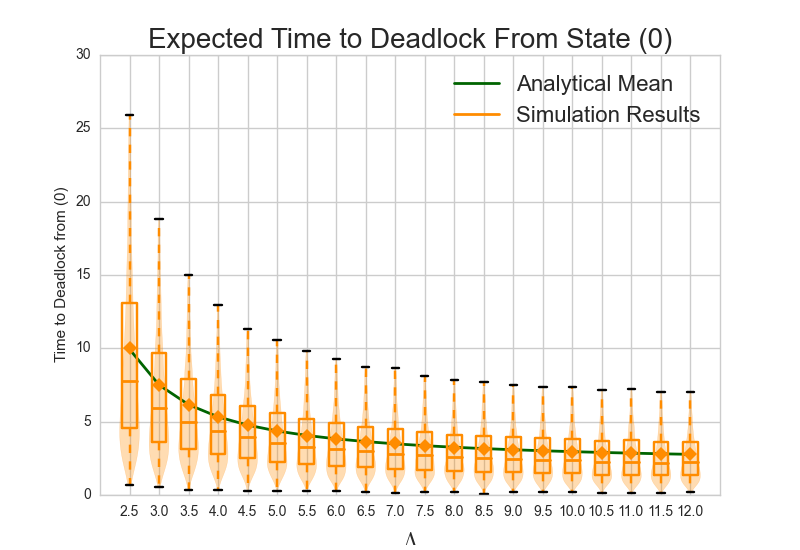
\includegraphics[width=\textwidth]{images/varyL_1Nms}
    \caption{Varying $\Lambda$}
    \label{fig:1Nms_L}
  \end{subfigure}
  \begin{subfigure}[b]{0.5\textwidth}
    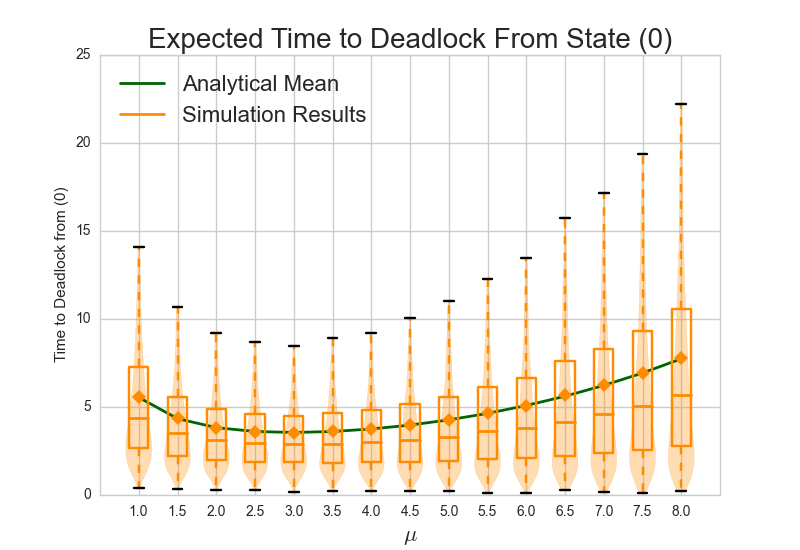
\includegraphics[width=\textwidth]{images/varymu_1Nms}
    \caption{Varying $\mu$}
    \label{fig:1Nms_mu}
  \end{subfigure}
  \begin{subfigure}[b]{0.5\textwidth}
    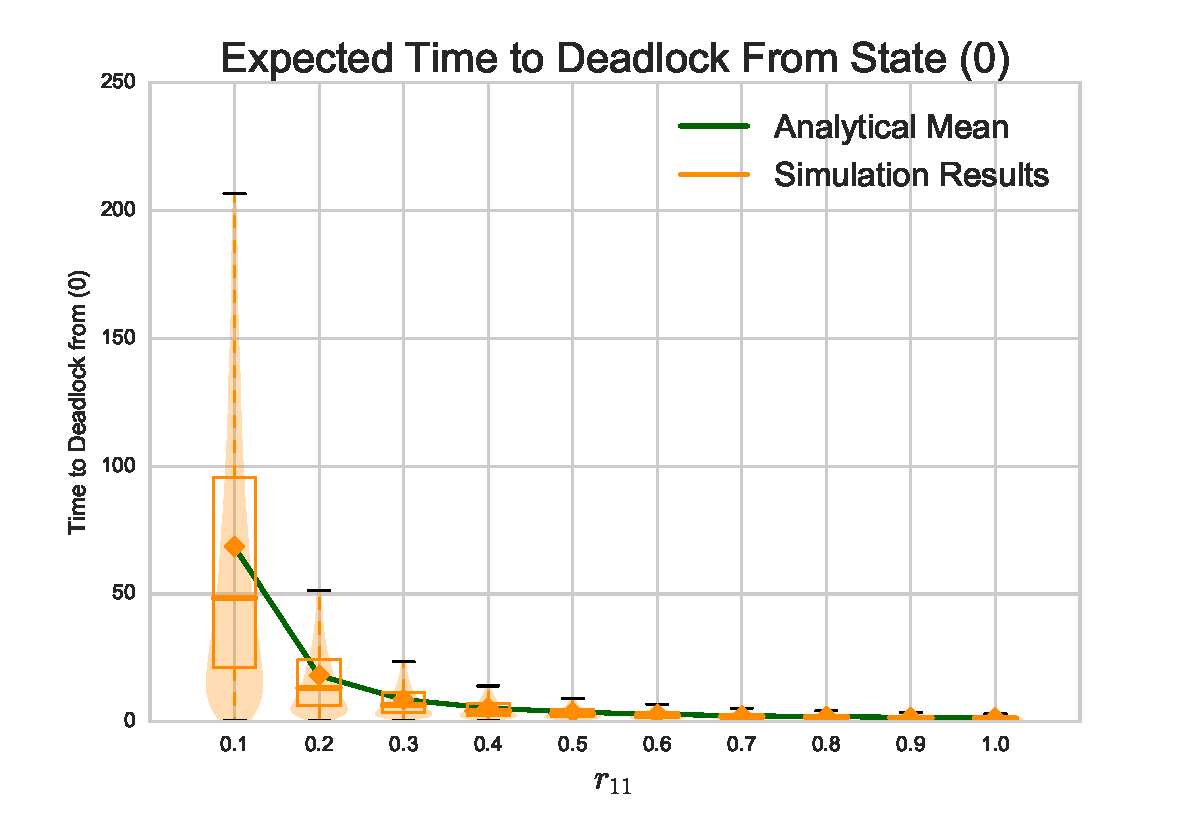
\includegraphics[width=\textwidth]{images/varyr11_1Nms}
    \caption{Varying $r_{11}$}
    \label{fig:1Nms_r11}
  \end{subfigure}
  \begin{subfigure}[b]{0.5\textwidth}
    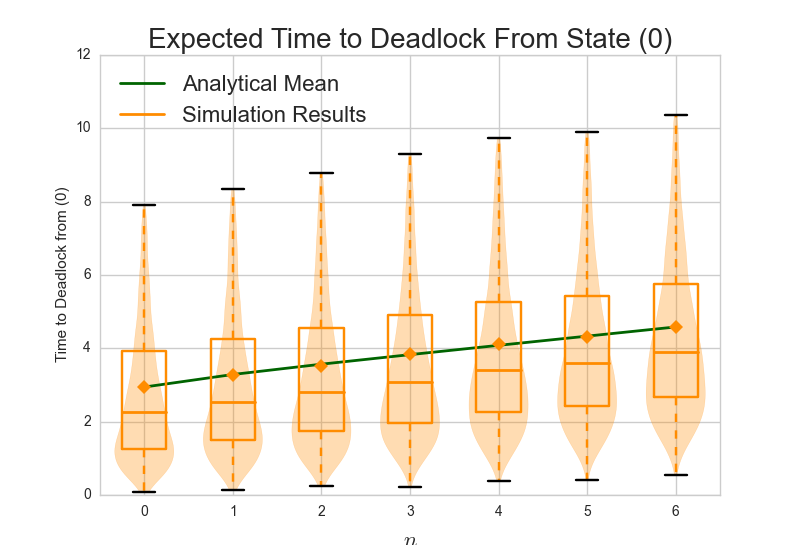
\includegraphics[width=\textwidth]{images/varyn_1Nms}
    \caption{Varying $n$}
    \label{fig:1Nms_n}
  \end{subfigure}
  \begin{center}
  \begin{subfigure}[b]{0.5\textwidth}
    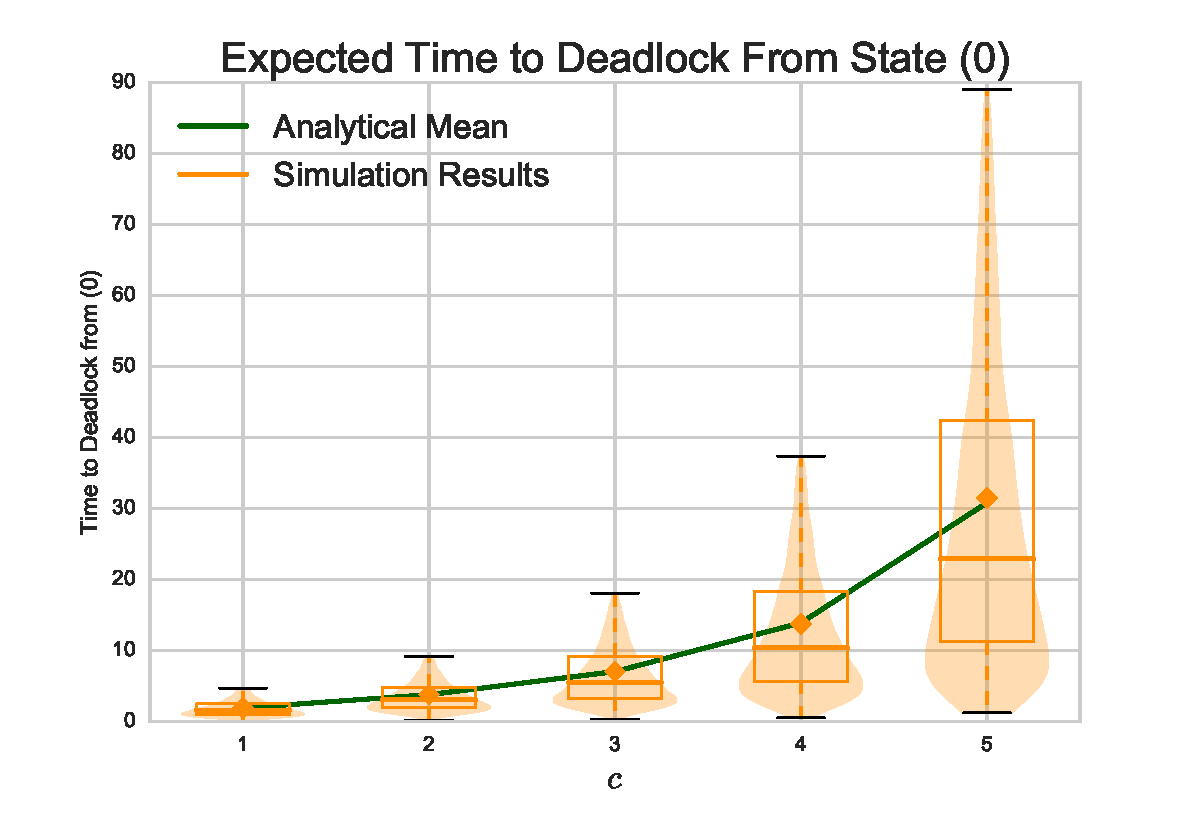
\includegraphics[width=\textwidth]{images/varyc_1Nms}
    \caption{Varying $c$}
    \label{fig:1Nms_c}
  \end{subfigure}
  \end{center}
  \caption{Time to deadlock in multi-server $\Omega_1$, analytical \& simulation results (10,000 iterations).}
  \label{fig:timestodeadlock1nodemultiserver}
\end{figure}


\subsubsection{Multi-Server: Two Node Network without Self Loops}\label{sec:2nodemulti}
Consider the two node network with feedback loops discussed in Subsection~\ref{sec:2nodewithoutselfloops}, now with $c_1$ parallel servers at the first node, and $c_2$ parallel servers at the second node.
This is shown in Figure~\ref{fig:queueingnetwork_2nodemulti}

\begin{figure}[!htbp]
  \includestandalone[width=\textwidth]{images/2nodemultiserver}
  \caption{A two node multi-server queueing network.}
  \label{fig:queueingnetwork_2nodemulti}
\end{figure}

State space:
        \[S = \{(i,j)\in\mathbb{N}^{(n_1+c_1+c_2)\times (n_2+c_2+c_1)} \nonscript\; | \nonscript\; i \leq n_1+c_1+j, \nonscript\; j \leq n_2+c_2+i\}\]
where $i$ denotes the number of individuals at Node 1 plus the number of individuals blocked waiting to enter Node 1, and $j$ denotes the number of individuals at Node 2 plus the number of individuals blocked waiting to enter Node 2.
For example, $(i, j) = (n_1+c_1+2, n_2+c_2+1)$ denotes a full system, $n_1+c_1$ individuals at Node 1, two of whom are blocked waiting to enter Node 2; $n_2+c_2$ individuals at Node 2, one of whom is blocked waiting to enter Node 1.
The state $(i, j) = (n_1+c_1+c_2, n_2+c_2+c_1)$ denotes the deadlocked state.

The Markov chain is shown in Figure~\ref{fig:2nodeMCms}.

\begin{figure}[!htbp]
    \includestandalone[width=\textwidth]{images/MC2nodemultiserv}
    \caption{Diagrammatic representation of the Markov chain for a multi server $\Omega_2$ system with $n_1=1$, $n_2=c_1=c_2=2$. The deadlocked state is $(5,6)$.}
    \label{fig:2nodeMCms}
\end{figure}

Define $\delta = (i_2, j_2) - (i_1, j_1)$, $b_1 = \max(0, i_1-n_1-c_1)$, $b_2 = \max(0, i_2-n_2-c_2)$, $s_1 = \min(i_1, c_1)-b_2$ and $s_2 = \min(i_2, c_2)-b_1$ ,then the transitions $q_{(i_1, j_1),(i_2, j_2)}$ are given by Table~\ref{tab:transitionsmultierv}.


\begin{table}
\begin{center}
\resizebox{\textwidth}{!}{
\begin{tabular}{ l | l | l | l |}
  & $j_1 < n_2 + c_2$ & $j_1 = n_2 + c_2$ & $ j_1 > n_2 + c_2$ \\ \hline
  \rotatebox[origin=c]{90}{$i_1 < n_1 + c_1$} & \begin{tabular}{ l } $\Lambda_1$ if $\delta = (1, 0)$ \\ $\Lambda_2$ if $\delta = (0, 1)$ \\ $r_{12}s_1\mu_1$ if $\delta = (-1, 1)$ \\ $r_{21}s_2\mu_2$ if $\delta = (1, -1)$ \\ $(1-r_{12})s_1\mu_1$ if $\delta = (-1, 0)$ \\ $(1-r_{21})s_2\mu_2$ if $\delta = (0, -1)$ \end{tabular} & \begin{tabular}{ l } $\Lambda_1$ if $\delta = (1, 0)$ \\ $r_{12}s_1\mu_1$ if $\delta = (0, 1)$ \\ $r_{21}s_2\mu_2$ if $\delta = (1, -1)$ \\ $(1-r_{12})s_1\mu_1$ if $\delta = (-1, 0)$ \\ $(1-r_{21})s_2\mu_2$ if $\delta = (0, -1)$ \end{tabular} & \begin{tabular}{ l } $\Lambda_1$ if $\delta = (1, 0)$ \\ $r_{12}s_1\mu_1$ if $\delta = (0, 1)$ \\ $r_{21}s_2\mu_2$ if $\delta = (0, -1)$ \\ $(1-r_{12})s_1\mu_1$ if $\delta = (-1, 0)$ \\ $(1-r_{21})s_2\mu_2$ if $\delta = (-1, -1)$ \end{tabular} \\ \hline
  \rotatebox[origin=c]{90}{$i_1 = n_1 + c_1$} & \begin{tabular}{ l } $\Lambda_2$ if $\delta = (0, 1)$ \\ $r_{12}s_1\mu_1$ if $\delta = (-1, 1)$ \\ $r_{21}s_2\mu_2$ if $\delta = (1, 0)$ \\ $(1-r_{12})s_1\mu_1$ if $\delta = (-1, 0)$ \\ $(1-r_{21})s_2\mu_2$ if $\delta = (0, -1)$ \end{tabular} & \begin{tabular}{ l } $r_{12}s_1\mu_1$ if $\delta = (0, 1)$ \\ $r_{21}s_2\mu_2$ if $\delta = (1, 0)$ \\ $(1-r_{12})s_1\mu_1$ if $\delta = (-1, 0)$ \\ $(1-r_{21})s_2\mu_2$ if $\delta = (0, -1)$ \end{tabular} & \begin{tabular}{ l } $r_{12}s_1\mu_1$ if $\delta = (0, 1)$ \\ $r_{21}s_2\mu_2$ if $\delta = (1, 0)$ \\ $(1-r_{12})s_1\mu_1$ if $\delta = (-1, 0)$ \\ $(1-r_{21})s_2\mu_2$ if $\delta = (-1, -1)$ \end{tabular} \\ \hline
  \rotatebox[origin=c]{90}{$i_1 > n_1 + c_1$} & \begin{tabular}{ l } $\Lambda_2$ if $\delta = (0, 1)$ \\ $r_{12}s_1\mu_1$ if $\delta = (-1, 0)$ \\ $r_{21}s_2\mu_2$ if $\delta = (1, 0)$ \\ $(1-r_{12})s_1\mu_1$ if $\delta = (-1, -1)$ \\ $(1-r_{21})s_2\mu_2$ if $\delta = (0, -1)$ \end{tabular} & \begin{tabular}{ l } $r_{12}s_1\mu_1$ if $\delta = (0, 1)$ \\ $r_{21}s_2\mu_2$ if $\delta = (1, 0)$ \\ $(1-r_{12})s_1\mu_1$ if $\delta = (-1, -1)$ \\ $(1-r_{21})s_2\mu_2$ if $\delta = (0, -1)$ \end{tabular} & \begin{tabular}{ l } $r_{12}s_1\mu_1$ if $\delta = (0, 1)$ \\ $r_{21}s_2\mu_2$ if $\delta = (1, 0)$ \\ $(1-r_{12})s_1\mu_1$ if $\delta = (-\min(b_1+1,b_2+1), -\min(b_1,b_2+1))$ \\ $(1-r_{21})s_2\mu_2$ if $\delta = (-\min(b_1+1,b_2), -\min(b_1+1,b_2+1))$ \end{tabular} \\ \hline
\end{tabular}
}
\caption{Table of transitions for a multi server two node network.}
\label{tab:transitionsmultierv}
\end{center}
\end{table}


The values $b_1$ and $b_2$ correspond to the number of people blocked to Node 1 and Node 2 respectively.
The values $s_1$ and $s_2$ correspond to the amount of people currently in service at Node 1 and Node 2 respectively.

This formulation of the Markov chain makes use of the following proposition:\\

\begin{proposition}
  In the two node queueing network described, if there are $b_1$ customers blocked to Node 1, and $b_2$ customers blocked to Node 2, where $b_1, b_2 > 0$, then:
  \begin{enumerate}[i.]
    \item \label{itm:exit1} A customer finishing service and leaving the system at Node 1 yields a difference in state of $\delta = (-\min(b_1+1, b_2+1), -\min(b_1, b_2+1))$.
    \item \label{itm:exit2} A customer finishing service and leaving the system at Node 2 yields a difference in state of $\delta = (-\min(b_1+1, b_2), -\min(b_1+1, b_2+1))$.
  \end{enumerate}
\end{proposition}

\begin{proof}
  Each new blocked individual contributes $(1, 1)$ to the state space. A blocked customer is counted as existing in the Node they are occupying, but also has a blocked part counted at the other node.

  Now an unblocking where a customer transitions from being blocked at Node 1 to being at Node 2 yields $\delta = (-1, 0)$; the customer's blocked part is no longer blocked, while they themselves transition to Node 2.
  This type of unblocking leaves space at Node 1 for more potential unblockings.

  Similarly an unblocking where a customer transitions from being blocked at Node 2 to being at Node 1 yields $\delta = (0, -1)$; the customer's blocked part is no longer blocked, while they themselves transition to Node 1.
  This type of unblocking leaves space at Node 2 for more potential unblockings.

  Consider a customer finishing service and exiting the system at Node 1.
  Breaking down the overall unblocking process into subprocesses, we can break down the overall difference $\delta$ into sub-differences $\delta_1$, $\delta_2$, $\delta_3$, etc, where $\delta = \sum_{i \in I} \delta_i$.

  The set $I$ is the number of sub-differences that happen until no more unblockings can happen.

  An unblockage at Node 1 always occurs after space at Node 2 is created, by an unblockage at Node 2.
  Therefore the maximium number of times a customer can be unblocked from Node 1 is either until there are no more blocked customers at Node 1, or no more unblockages at Node 2, as there are no more customers at Node 2 to unblock.
  Therefore $\min(b_1, b_2)$ unblockages of this kind.

  An unblockage at Node 2 occurs after an unblockage at Node 1 if there are enough blocked customers to do so.
  An unblockage at Node 2 causes an unblockage at Node 1, and so directly proceeds an unblockage at Node 1.
  If $b_2 > b_1$ there are $b_1$ unblockages at Node 1, and so $b_1$ unblockages at Node 2.
  If $b_1 > b_2$ there are $b_2$ unblockages at Node 1, and so $b_2+1$ unblockages at Node 2.
  Therefore $\min(b_1, b_2+1)$ unblockages of this kind.

  Now:
  \begin{align*}
    \delta &= \sum_{i \in I} \delta_i\\
    &= (-1, 0) + (0, -1) + (-1, 0) + (0, -1) + \dots\\
    &= (-1, 0) + \min(b_1, b_2+1)\times(0, -1) + \min(b_2, b_1)\times(-1, 0)\\
    &= (-\min(b_1+1, b_2+1), -\min(b_1, b_2+1))
  \end{align*}

  A similar argument yields $\delta = (-\min(b_1+1, b_2), -\min(b_1+1, b_2+1))$ for the situation where a customer finishes service at Node 2 and exits the system.

\end{proof}

Figure~\ref{fig:timestodeadlock2nodemultiserver} shows the effect of varying the parameters of the above Markov model.
Base parameters of $\Lambda_1 = 9$, $\Lambda_2 = 7.5$, $n_1 = 2$, $n_2 = 1$, $\mu_1 = 5.5$, $\mu_2 = 6.5$, $r_{12} = 0.7$, $r_{21} = 0.6$, $c_1 = 2$ and $c_2 = 2$ were used.

\begin{figure}[!htbp]
  \begin{subfigure}[b]{0.333\textwidth}
    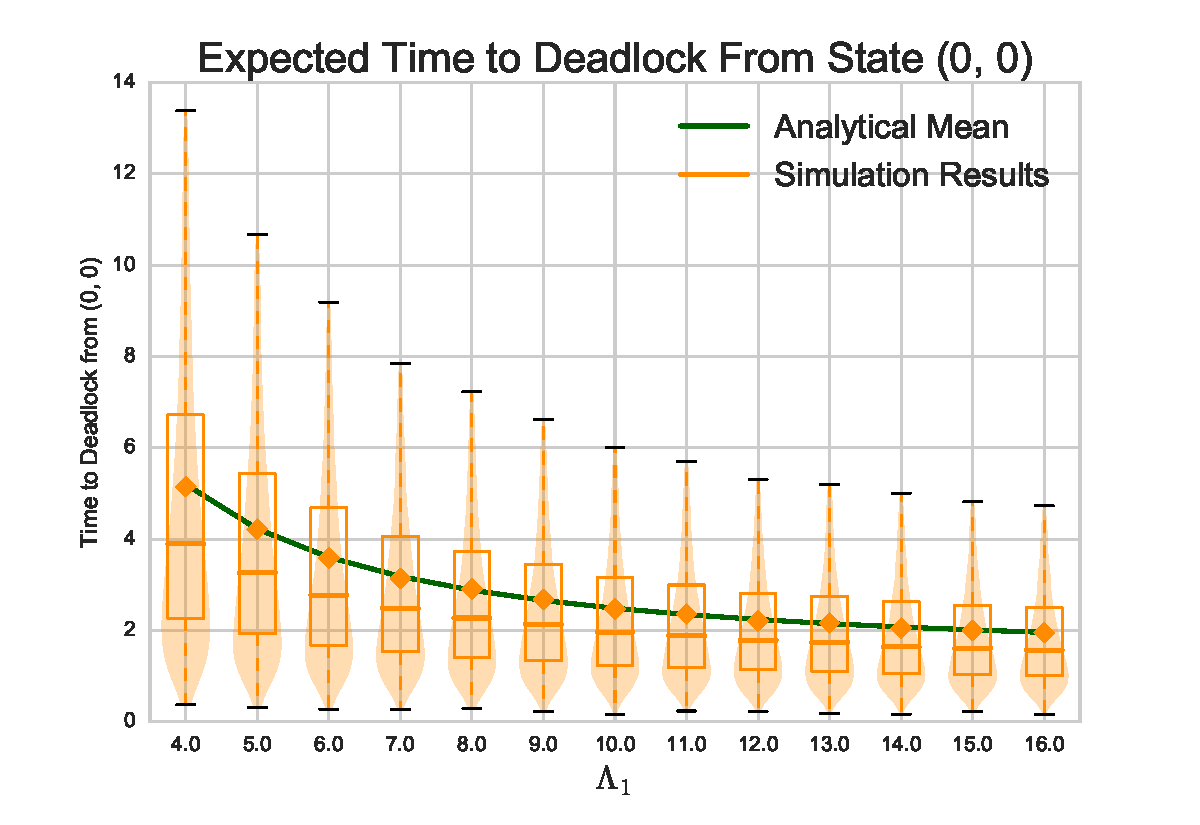
\includegraphics[width=\textwidth]{images/varyL1_2Nms}
    \caption{Varying $\Lambda_1$}
    \label{fig:2Nms_L1}
  \end{subfigure}
  \begin{subfigure}[b]{0.333\textwidth}
    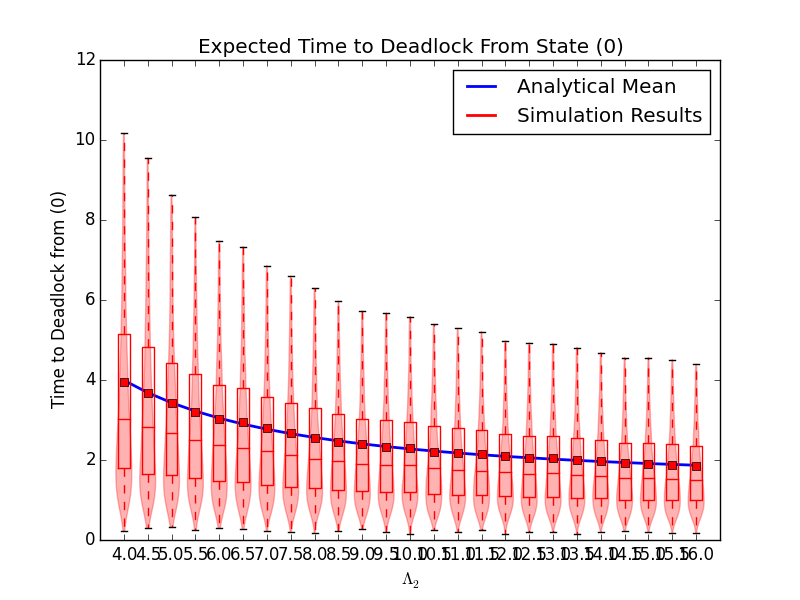
\includegraphics[width=\textwidth]{images/varyL2_2Nms}
    \caption{Varying $\Lambda_@$}
    \label{fig:2Nms_L2}
  \end{subfigure}
  \begin{subfigure}[b]{0.333\textwidth}
    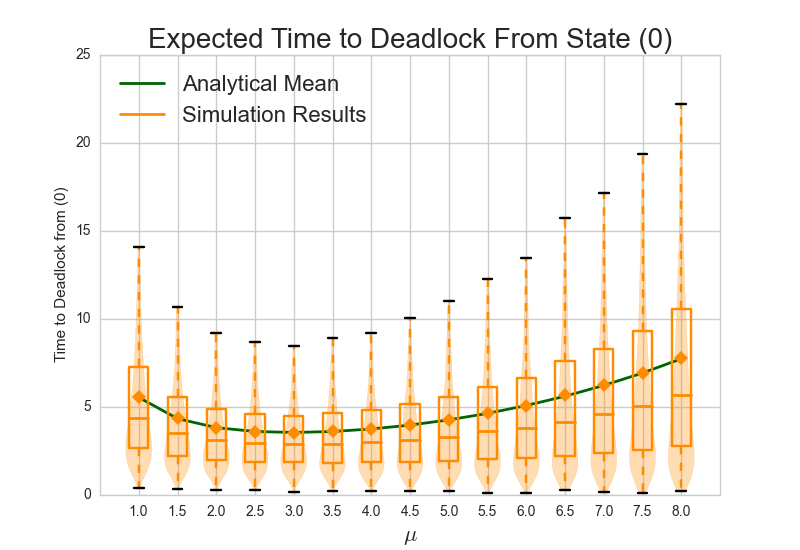
\includegraphics[width=\textwidth]{images/varymu_1Nms}
    \caption{Varying $\mu_1$}
    \label{fig:2Nms_mu1}
  \end{subfigure}
  \begin{subfigure}[b]{0.333\textwidth}
    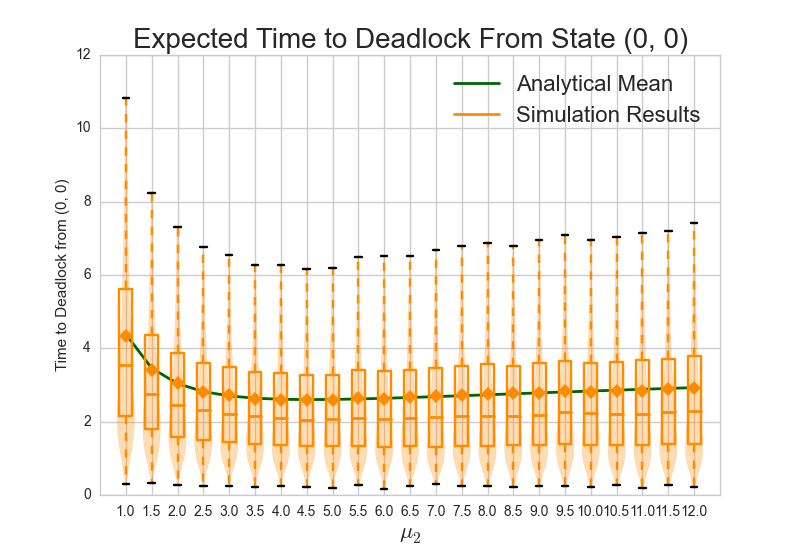
\includegraphics[width=\textwidth]{images/varymu2_2Nms}
    \caption{Varying $\mu_2$}
    \label{fig:2Nms_mu2}
  \end{subfigure}
  \begin{subfigure}[b]{0.333\textwidth}
    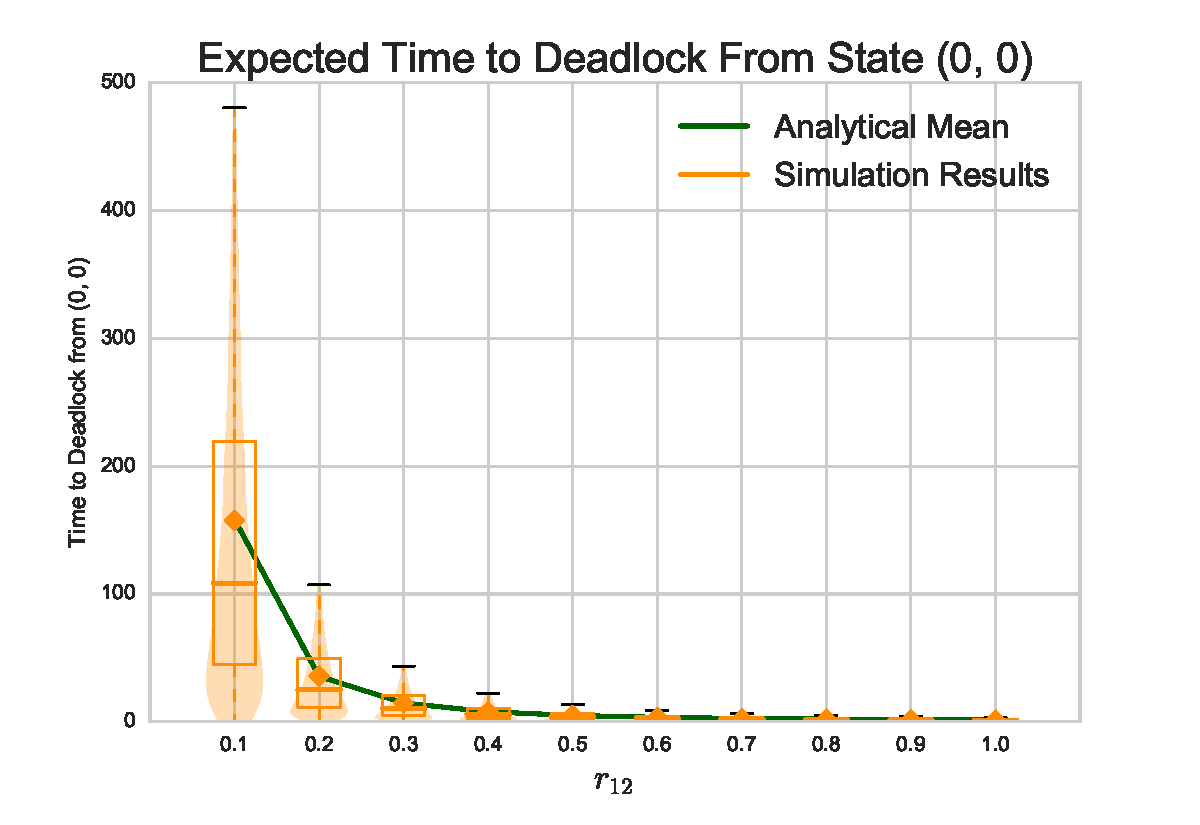
\includegraphics[width=\textwidth]{images/varyr12_2Nms}
    \caption{Varying $r_{12}$}
    \label{fig:2Nms_r12}
  \end{subfigure}
  \begin{subfigure}[b]{0.333\textwidth}
    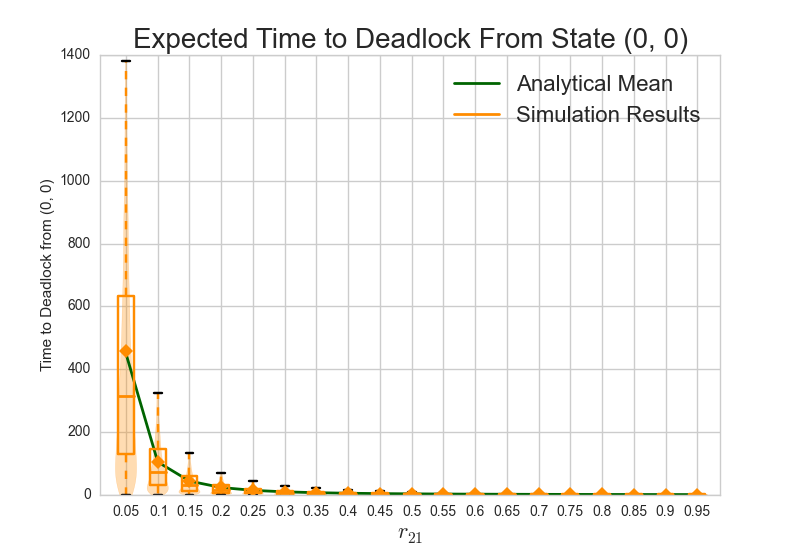
\includegraphics[width=\textwidth]{images/varyr21_2Nms}
    \caption{Varying $r_{21}$}
    \label{fig:2Nms_r21}
  \end{subfigure}
  \begin{center}
  \begin{subfigure}[b]{0.34\textwidth}
    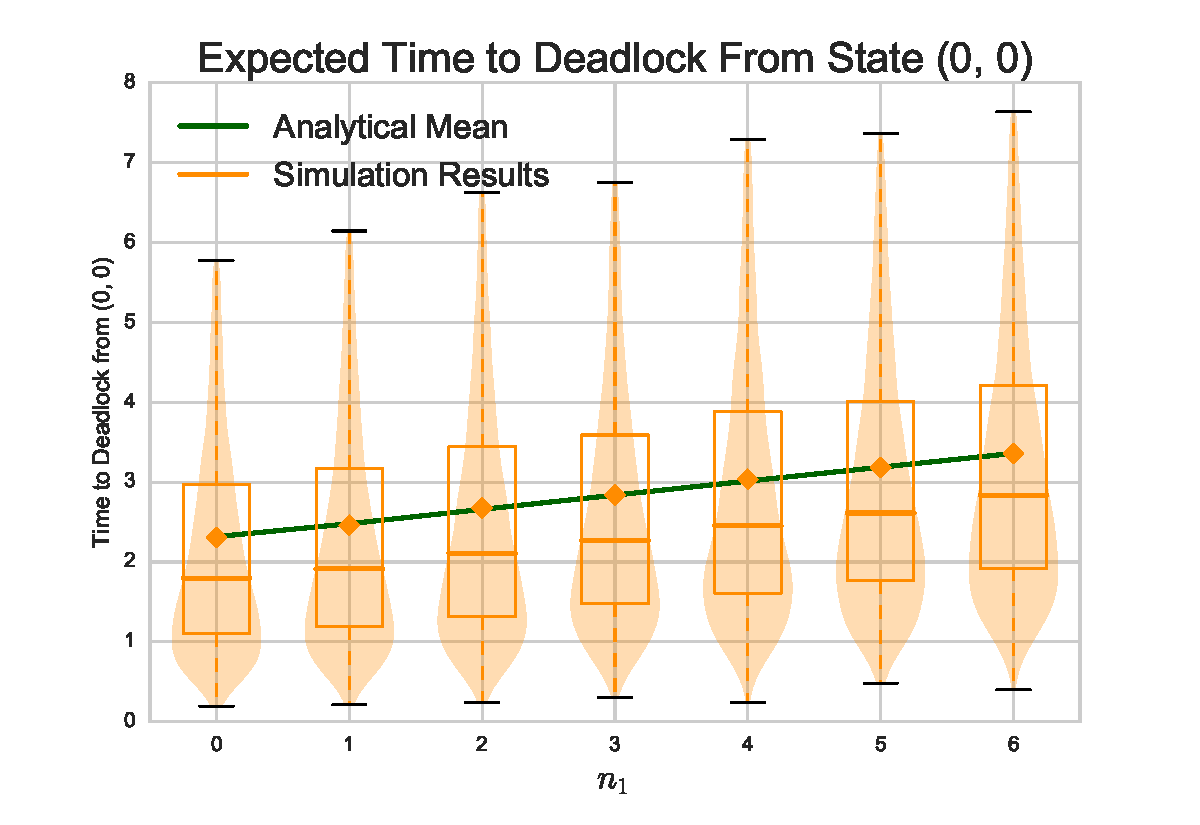
\includegraphics[width=\textwidth]{images/varyn1_2Nms}
    \caption{Varying $n_1$}
    \label{fig:2Nms_n1}
  \end{subfigure}
  \begin{subfigure}[b]{0.34\textwidth}
    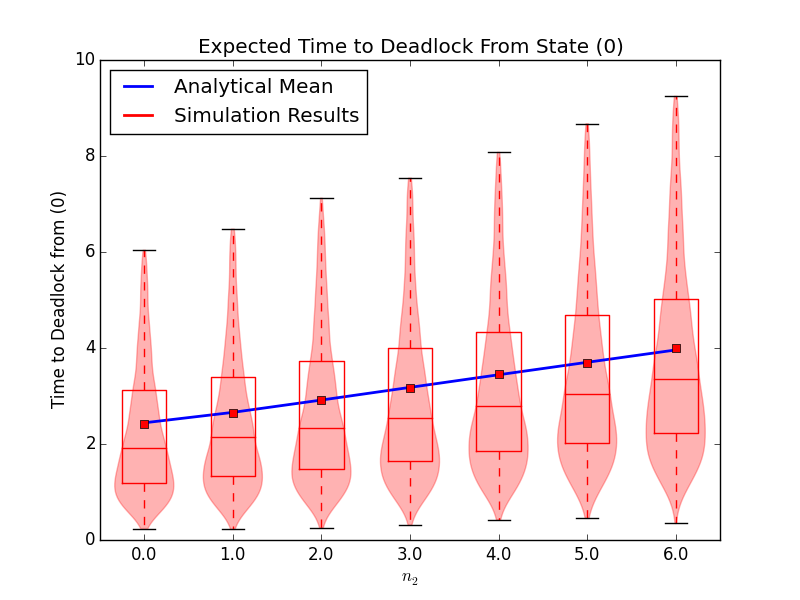
\includegraphics[width=\textwidth]{images/varyn2_2Nms}
    \caption{Varying $n_2$}
    \label{fig:2Nms_n2}
  \end{subfigure}
  \begin{subfigure}[b]{0.34\textwidth}
    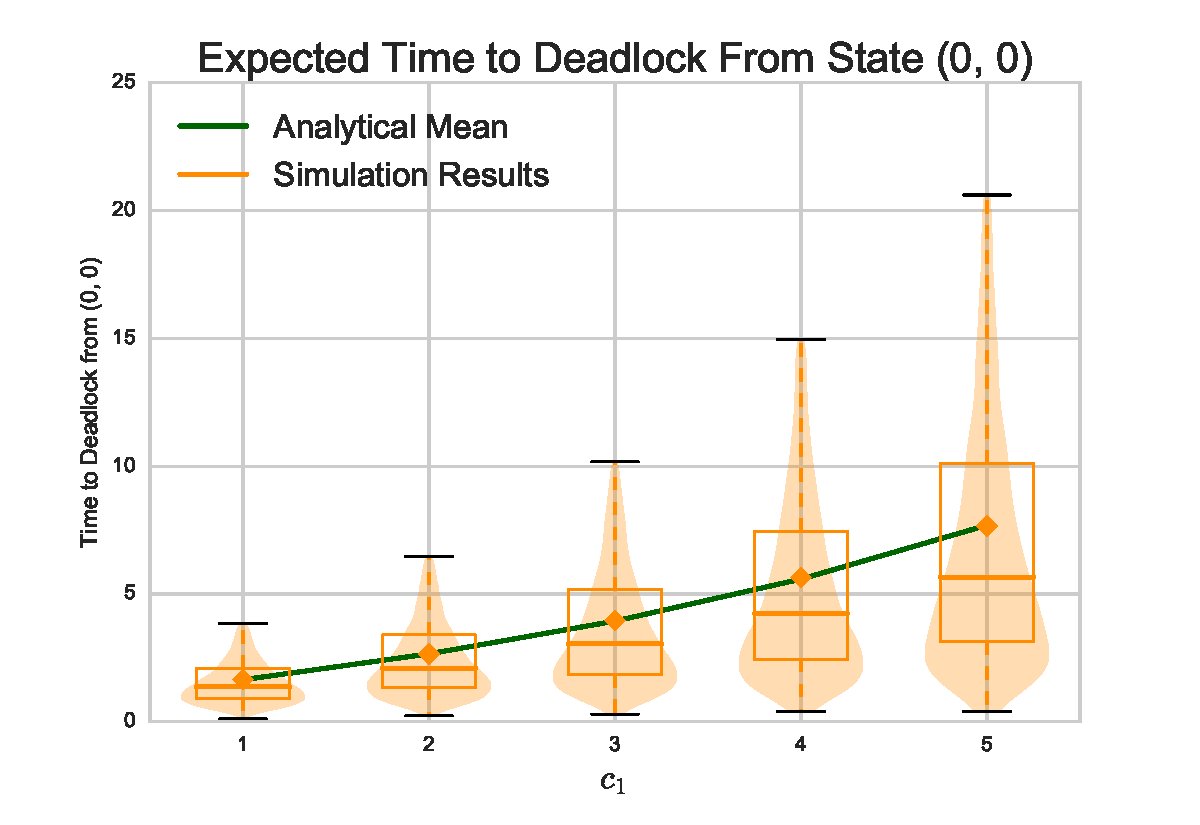
\includegraphics[width=\textwidth]{images/varyc1_2Nms}
    \caption{Varying $c_1$}
    \label{fig:2Nms_c1}
  \end{subfigure}
  \begin{subfigure}[b]{0.34\textwidth}
    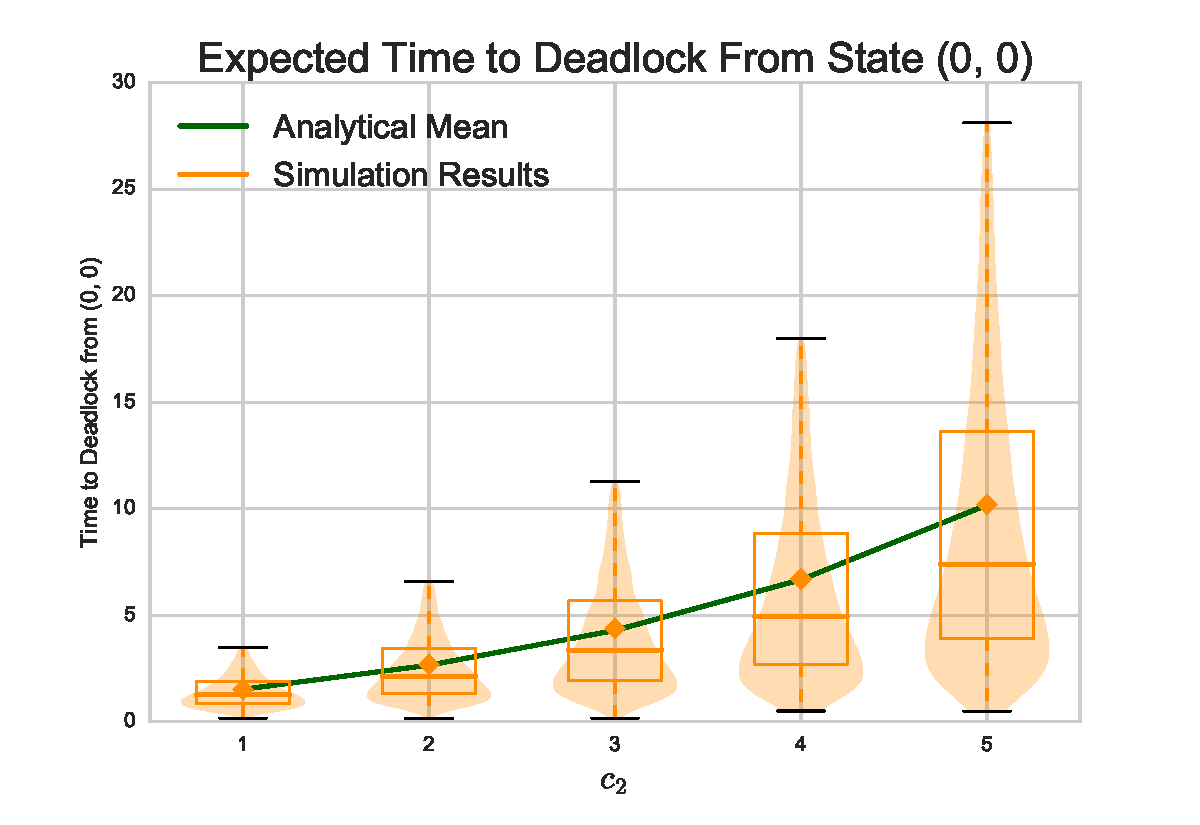
\includegraphics[width=\textwidth]{images/varyc2_2Nms}
    \caption{Varying $c_2$}
    \label{fig:2Nms_c2}
  \end{subfigure}
  \end{center}
  \caption{Time to deadlock in multi-server $\Omega_2$, analytical \& simulation results (10,000 iterations).}
  \label{fig:timestodeadlock2nodemultiserver}
\end{figure}




\section{A Bound on the Mean Time to Deadlock}\label{sec:bound}
This section will derive a bound for the mean time to deadlock of the $\Omega$ system.
In order to do this, six deadlocking queueing networks are defined as follows:

\begin{itemize}
  \item Define $\Omega_{1_1}^{\star}$ as the 1 node queueing network described in Subsection~\ref{sec:1nodenet} with the parameter set $(\Lambda_1$, $\mu_1$, $n_1$, $r_{11})$. Let its mean time to deadlock be denoted by $\omega_{1_1}^{\star}$.
  \item Define $\Omega_{1_1}^{\star\star}$ as the 1 node queueing network described in Subsection~\ref{sec:1nodenet} with the parameter set $(\Lambda_1$, $m_1$, $n_1$, $r_{11})$. Let its mean time to deadlock be denoted by $\omega_{1_1}^{\star\star}$.
  \item Define $\Omega_{1_2}^{\star}$ as the 1 node queueing network described in Subsection~\ref{sec:1nodenet} with the parameter set $(\Lambda_2$, $\mu_2$, $n_2$, $r_{22})$. Let its mean time to deadlock be denoted by $\omega_{1_2}^{\star}$.
  \item Define $\Omega_{1_2}^{\star\star}$ as the 1 node queueing network described in Subsection~\ref{sec:1nodenet} with the parameter set $(\Lambda_2$, $m_2$, $n_2$, $r_{22})$. Let its mean time to deadlock be denoted by $\omega_{1_2}^{\star\star}$.
  \item Define $\Omega_2$ as the 2 node queueing network described in Subsection~\ref{sec:2nodewithoutselfloops} with the parameter set $(\Lambda_1$, $\Lambda_2$, $\mu_1$, $\mu_2$, $n_1$, $n_2$, $r_{12}$, $r_{21})$. Let its mean time to deadlock be denoted by $\omega_2$.
  \item Define $\Omega$ as the 2 node queueing network described in Subsection~\ref{sec:2nodeselfloops} with the parameter set $(\Lambda_1$, $\Lambda_2$, $\mu_1$, $\mu_2$, $n_1$, $n_2$, $r_{11}$, $r_{12}$, $r_{21}$, $r_{22})$. Let its mean time to deadlock be denoted by $\omega$.
\end{itemize}
where $m_1 = \frac{\mu_2}{3 + 2\frac{\mu_2}{\mu_1} + \frac{\mu_1}{\mu_2}}$, and $m_2 = \frac{\mu_1}{3 + 2\frac{\mu_1}{\mu_2} + \frac{\mu_2}{\mu_1}}$.

Figure~\ref{fig:decomposeqnet} shows how $\Omega$ contains, and is made up by, $\Omega_{1_1}$, $\Omega_{1_2}$ and $\Omega_2$.

\begin{figure}[!htbp]
\begin{subfigure}[b]{0.5\textwidth}
  \includestandalone[width=\textwidth]{images/omega11}
  \caption{$\Omega_{1_1}$ within $\Omega$}
  \label{fig:omega11withinomega}
\end{subfigure}
\begin{subfigure}[b]{0.5\textwidth}
  \includestandalone[width=\textwidth]{images/omega12}
  \caption{$\Omega_{1_2}$ within $\Omega$}
  \label{fig:omega12withinomega}
\end{subfigure}
\begin{center}
\begin{subfigure}[b]{0.5\textwidth}
  \includestandalone[width=\textwidth]{images/omega2}
  \caption{$\Omega_2$ within $\Omega$}
  \label{fig:omega2withinomega}
\end{subfigure}
\end{center}
\caption{Decomposition of $\Omega$ into $\Omega_{1_1}$, $\Omega_{1_2}$ and $\Omega_2$}
\label{fig:decomposeqnet}
\end{figure}

Defining $\omega_{1_j} = \max(\omega_{1_j}^{\star}, \omega_{1_j}^{\star\star})$ we get the following bound:\\

\begin{theorem}
For any parameter sets the following inequality holds:
$\omega \leq \min(\omega_{1_1}, \omega_{1_2}, \omega_2)$
\end{theorem}

\begin{proof}
First, define the following systems:
\begin{itemize}
  \item Let $\widetilde{\Omega}_{1_1}$ denote the $\Omega_{1_1}$ system embedded within $\Omega$. Let $\widetilde{\omega}_{1_1}$ denote the mean time to deadlock of $\widetilde{\Omega}_{1_1}$.
  \item Let $\widetilde{\Omega}_{1_2}$ denote the $\Omega_{1_2}$ system embedded within $\Omega$. Let $\widetilde{\omega}_{1_2}$ denote the mean time to deadlock of $\widetilde{\Omega}_{1_2}$.
  \item Let $\widetilde{\Omega}_2$ denote the $\Omega_2$ system embedded within $\Omega$. Let $\widetilde{\omega}_2$ denote the mean time to deadlock of $\widetilde{\Omega}_2$.
\end{itemize}

Now $\widetilde{\omega}_{1_1}$ is the mean time to state (-1) in $\Omega$, $\widetilde{\omega}_{1_2}$ is the mean time to state (-2) in $\Omega$ and $\widetilde{\omega}_2$ is the mean time to state (-3) in $\Omega$.
Therefore $\omega = \min(\widetilde{\omega}_{1_1}, \widetilde{\omega}_{1_2}, \widetilde{\omega}_2)$, as the mean time to deadlock in $\Omega$ is the expected time it takes to reach either (-1), (-2) or (-3), whichever comes first.

Comparing $\widetilde{\Omega}_2$ to $\Omega_2$:
The effective arrival rate to Node 1 in $\widetilde{\Omega}_2$ is greater than or equal to the effective arrival rate to Node 1 in $\Omega_2$.
This is due to the extra customers who are rejoining the queue after service.
Similarly the effective arrival rate to Node 2 in $\widetilde{\Omega}_2$ is greater than or equal to the effective arrival rate to Node 2 in $\Omega_2$.
As an increase in the arrival rate causes the mean time to deadlock to decrease, we can conclude $\widetilde{\omega}_2 \leq \omega_2$

Consider $\widetilde{\Omega}_{1_1}$.
Consider the expected effective service time, the time that $\widetilde{\Omega}_{1_1}$'s state does not change due to services or outside factors.

The shortest expected effective service time is equal to $\frac{1}{\mu_1}$, corresponding to when neither Node 1 nor Node 2 are full.
Therefore the largest effective service rate is $\mu_1$.

The longest service time corresponds to when Node 2 is full, Node 1 finishes service and gets blocked.
Here the customer in service at Node 1 spends $\frac{1}{\mu_1}$ in service, then gets blocked.
That customer remains blocked until there is room at Node 2, that is when Node 2 has a service.
As all service rates are Markovian, the time spent blocked is $\frac{1}{\mu_2}$.

If the customer finishing service at Node 2 transitions to Node 1, then $\widetilde{\Omega}_{1_1}$'s state hasn't changed, and Node 2 is full again.
The next customer at Node 1 now spends $\frac{1}{\mu_1}$ in service.
This process will repeat if Node 1 is blocked before Node 2 releases a customer, and so the process is repeated with probability $P_{\text{repeat}}$.

And so the longest effective service time is:

\begin{align*}
  \frac{1}{m_1} & = \frac{2}{\mu_1} + \frac{1}{\mu_2} + P_{\text{repeat}} \left( \frac{2}{\mu_1} + \frac{1}{\mu_2} + P_{\text{repeat}} \left( \frac{2}{\mu_1} + \frac{1}{\mu_2} + P_{\text{repeat}} \bigg( \dotsi \right. \right. \\
  & = \left( \frac{2}{\mu_1} + \frac{1}{\mu_2} \right) \times \left( 1 + P_{\text{repeat}} + P_{\text{repeat}}^2 + P_{\text{repeat}}^3 + \dots \right) \\
  & = \left( \frac{2}{\mu_1} + \frac{1}{\mu_2} \right) \times \left( \frac{1}{1 - P_{\text{repeat}}} \right)
\end{align*}

If $S_1$ is the time the customer at Node 1 spends in service, and $S_2$ is the time the customer at node 2 spends in service, then $S_1 \sim \text{Exp}(\mu_1)$ and $S_2 \sim \text{Exp}(\mu_2)$.
Now $P_{\text{repeat}} = P(S_1 < S_2) = \frac{\mu_1}{\mu_1 + \mu_2}$.

Therefore the smallest effective service rate is:

\begin{align*}
  m_1 & = \frac{1}{ \left( \frac{2}{\mu_1} + \frac{1}{\mu_2} \right) \left( \frac{1}{1-P_{\text{repeat}}} \right) } \\
  & = \frac{1}{ \left( \frac{2}{\mu_1} + \frac{1}{\mu_2} \right) \left( \frac{1}{1-\frac{\mu_1}{\mu_1 + \mu_2}} \right) } \\
  & = \frac{1}{ \left( \frac{2}{\mu_1} + \frac{1}{\mu_2} \right) \left( \frac{\mu_1 + \mu_2}{\mu_2} \right) } \\
  & = \frac{\mu_2}{ \left( \frac{2}{\mu_1} + \frac{1}{\mu_2} \right) \left( \mu_1 + \mu_2 \right) } \\
  & = \frac{\mu_2}{3 + 2\frac{\mu_2}{\mu_1} + \frac{\mu_1}{\mu_2}} \\
\end{align*}

As time to deadlock does not increase monotonically with service rate (see Figure~\ref{fig:timestodeadlock_mu}) we cannot simply compare $\widetilde{\Omega}_{1_1}$ with the system that has the largest of smallest service rate; instead we must compare $\widetilde{\Omega}_{1_1}$ with either the system with the smallest service rate or the largest, whichever yields the longest time to deadlock.

The largest service rate is $\mu_1$, corresponding to system $\Omega_{1_1}^{\star}$ and the smallest is $m$ corresponding to $\Omega_{1_1}^{\star\star}$.
And so we compare with whichever system takes longer to reach deadlock. Using Lemma~\ref{lem:oneminima} and Remark~\ref{rem:findmaximum} we compare with $\omega_{1_1} = \max(\omega_{1_1}^{\star}, \omega_{1_1}^{\star\star})$.

And so comparing this to $\widetilde{\Omega}_{1_1}$: the effective arrival rate in $\widetilde{\Omega}_{1_1}$ is greater than or equal to the effective arrival rate in that system; this is due to the extra customers who have transitioned from the Node 2 to Node 1. An increase in the arrival rate causes the mean time to deadlock to decrease.

We can conclude that $\widetilde{\omega}_{1_1} \leq \omega_{1_1}$ at $\widetilde{\omega}_{1_1}$'s worst case scenrio, and so $\widetilde{\omega}_{1_1} \leq \omega_{1_1}$ in general.

Similarly we can conclude $\widetilde{\omega}_{1_2} \leq \omega_{1_2}$.

And so

\begin{align*}
\min(\widetilde{\omega}_{1_1}, \widetilde{\omega}_{1_2}, \widetilde{\omega}_2) &\leq \min(\omega_{1_1}, \omega_{1_2}, \omega_2) \\
\omega &\leq \min(\omega_{1_1}, \omega_{1_2}, \omega_2)
\end{align*}

\end{proof}


% \section{Resolving Deadlock}
% Once the system falls into a deadlocked state for the first time, that is the first transient deadlocked state since the last resolution, the simulated needs to automatically resolve the deadlock and allow services to resume again.
% This is not necessarily as simple as moving a blocked customer to his next node, as we need to conserve the numbers of customers at each service station.
% Closer inspection of the state digraph is required in order to find a way to resolve deadlock whilst conserving this property.

% At deadlock, the service stations can be classified into the following three mutually exclusive categories:
% \begin{itemize}
%     \item Nodes that are not deadlocked: These are nodes that do not contain any blocked individuals.
%     \item Causation nodes, nodes causing deadlock: These are nodes where every server is occupied by a blocked individual, and there is at least one blocked individual waiting to enter that node who is directly or indirectly being blocked by an individual in this node.
%     \item Affected nodes, nodes affected by deadlock: These are nodes containing at least one blocked individual who is directly or indirectly being blocked by an individual at a node that is causing deadlock, but is not classified as causing deadlock itself.
% \end{itemize}

% At the first instance of deadlock, there will only be one knot in $D(t)$.
% Let us denote the knot as $K$.
% The vertices of $K$ correspond to servers.
% As there is no sink node, all vertices of $K$ have an out-edge, and so all vertices in $K$ contain a blocked individual.
% Therefore, there are no vertices in $K$ belonging to nodes that are not deadlocked.
% All vertices of $K$ correspond to servers of causation nodes, and a causation node has all its servers belonging to $K$.
% An affected node has servers belonging to the same weakly connected component as $K$, but does not have servers in $K$.

% When choosing which customer to move in order to resolve deadlock, we must be careful to conserve the number of customers at each service station.
% Causation nodes have full queues, and a customer may only be moved into a full queue if this causes another customer to simultaneously move from this node.
% Another complication arises due to the blocking mechanism used, in which those customers who have been blocked longer must be moved first.
% This property may have to be broken in order to ensure the conservation property is not.
% Assume that we have weighted the edges of the digraph with the time that they were created. % If this works then I'll include this in the write up of how state digraph is formed

% The following algorithm is proposed in order to resolve deadlock:

% \begin{algorithm}[H]
%     \DontPrintSemicolon
%     Find the knot $K$ in $D(t)$\;
%     Find the cycle $C \in K$ whose average edge weight is minimum\;
%     Start at $V_0$\;
%     \For{$V_i$ in $C$}{
%     Move the individual who is waiting to get to $V_{i+1}$\;}
%     Redraw $D(t)$\;
% \end{algorithm}



\bibliographystyle{plain}
\bibliography{refs}

\section*{Appendix}
Some definitions from graph theory that have been used in this report:

\begin{itemize}
  \item \textbf{Order}: The order of the directed graph $D$ is its number of vertices, denoted by $\left| V(D) \right|$.
  \item \textbf{Weakly connected component}: A weakly connected component of a digraph containing $X$ is the set of all nodes that can be reached from $X$ if we ignore the direction of the edges.
  \item \textbf{Direct successor}: If a directed graph contains an edge from $X_i$ to $X_j$ , then we say that $X_j$ is a direct successor of $X_i$.
  \item \textbf{Ancestors}: If a directed graph contains a path from $X_i$ to $X_j$ , then we say that $X_i$ is an ancestor of $X_j$.
  \item \textbf{Descendants}: If a directed graph contains a path from $X_i$ to $X_j$ , then we say that $X_j$ is a descendant of $X_i$.
  \item \textbf{$\text{deg}^{\text{out}}(X)$}: The out-degree of $X$ is the number of outgoing edges emanating from that vertex.
  \item \textbf{Subgraph}: A subgraph $H$ of a graph $G$ is a graph whose vertices are a subset of the vertex set of $G$, and whose edges are a subset of the edge set of $G$.
  \item \textbf{Sink vertex}: A sink vertex is a vertex in a directed graph that has out-degree of zero.
  \item \textbf{Knot}: In a directed graph, a knot is a set of vertices with out-edges such that while traversing the directed edges of that directed graph, once a vertex in the knot is reached, you cannot reach any vertex that is not in the knot.
\end{itemize}

\end{document}
